\documentclass[12pt,a4paper]{report}

% -------------------------
% PACKAGES
% -------------------------
\usepackage[margin=1in]{geometry}
\usepackage{setspace}
% \usepackage{times} % Times New Roman
\usepackage{newtxtext,newtxmath}
\usepackage[utf8]{inputenc}
\usepackage[T1]{fontenc}
\usepackage{graphicx}
\usepackage{titlesec}
\usepackage{tocloft}
\usepackage{indentfirst}
\usepackage{fancyhdr}
\usepackage{ragged2e}
\usepackage{hyperref}
% \usepackage{apacite}
\usepackage[style=apa, backend=biber]{biblatex}
\addbibresource{references.bib}
\usepackage{tikz}
\usetikzlibrary{positioning} % Required for "below=of" syntax
\usepackage{float} % Required for the [H] figure placement
\usepackage{xcolor}
\usepackage{listings}
\usepackage{booktabs}
\usepackage{tabularx}
\usepackage{enumitem}
% \usepackage{titlesec}
\usetikzlibrary{positioning, arrows.meta}
\usepackage{afterpage}
\usepackage{url}
\usepackage{etoolbox}
\usepackage{caption}


% Remove indentation for List of Figures
\setlength{\cftfigindent}{0pt}      % Sets the indent to 0
\setlength{\cftfignumwidth}{2.3em}  % Adjusts space for the "Figure 1.1" label

% Remove indentation for List of Tables
\setlength{\cfttabindent}{0pt}      % Sets the indent to 0
\setlength{\cfttabnumwidth}{2.3em}  % Adjusts space for the "Table 1.1" label

\makeatletter
% \usepackage[breaklinks]{hyperref}
% \usepackage{ulem}

% Define custom colors
\definecolor{codegreen}{rgb}{0,0.6,0}
\definecolor{codegray}{rgb}{0.5,0.5,0.5}
\definecolor{codepurple}{rgb}{0.58,0,0.82}
\definecolor{backcolour}{rgb}{0.95,0.95,0.92}


% Reduce spacing around display math
\setlength{\abovedisplayskip}{0pt}
\setlength{\belowdisplayskip}{0pt}
\setlength{\abovedisplayshortskip}{0pt}
\setlength{\belowdisplayshortskip}{0pt}

% For equations in itemize/enumerate environments:
\makeatletter
\g@addto@macro\normalsize{%
  \setlength\abovedisplayskip{0pt}
  \setlength\belowdisplayskip{0pt}
  \setlength\abovedisplayshortskip{0pt}
  \setlength\belowdisplayshortskip{0pt}
}
\makeatother

% % Configure list environments to match paragraph indent
% \setlist[itemize]{
%   leftmargin=0.5in,    % Align with paragraph indent
%   itemindent=0pt,      % No extra indent for item
%   labelsep=0.3em,      % Space between bullet and text
%   topsep=3pt,          % Space before list
%   partopsep=0pt,       % No extra space if starting new paragraph
%   parsep=6pt,          % Space between items
%   itemsep=6pt,         % Space between items
% }

% \setlist[enumerate]{
%   leftmargin=0.5in,
%   itemindent=0pt,
%   labelsep=0.3em,
%   topsep=6pt,
%   partopsep=0pt,
%   parsep=6pt,
%   itemsep=6pt,
% }

\setlist[itemize]{
  leftmargin=*,
  itemindent=0pt,
  labelsep=0.5em,
  topsep=6pt,
  partopsep=0pt,
  parsep=6pt,
  itemsep=6pt,
}

\setlist[enumerate]{
  leftmargin=*,
  itemindent=0pt,
  labelsep=0.5em,
  topsep=6pt,
  partopsep=0pt,
  parsep=6pt,
  itemsep=6pt,
}

% % Configure list environments to align bullets with paragraph indents
% \setlist[itemize]{
%   leftmargin=0.5in,         % This aligns the bullet (label) at the 0.5in mark
%   labelsep=0.5em,           % Space between bullet and text
%   align=left,               % Ensures the label is pushed to the left of the margin
%   nosep,                    % Single-spaced (as we discussed before)
%   % after=\vspace{\baselineskip} % Adds a double-space gap after the list
% }

% \setlist[enumerate]{
%   leftmargin=0.5in,         % Aligns the number at the 0.5in mark
%   labelsep=0.5em,
%   align=left,
%   nosep,
%   % after=\vspace{\baselineskip}
% }


% Global style configuration
\lstset{
  backgroundcolor=\color{backcolour},
  commentstyle=\color{codegreen},
  keywordstyle=\color{magenta},
  numberstyle=\tiny\color{codegray},
  stringstyle=\color{codepurple},
  basicstyle=\ttfamily\footnotesize,
  breakatwhitespace=false,
  breaklines=true,
  captionpos=b,
  keepspaces=true,
  numbers=left,
  numbersep=5pt,
  showspaces=false,
  showstringspaces=false,
  showtabs=false,
  tabsize=2
}

% -------------------------
% NEW COMMANDS
% -------------------------

\newcommand{\LogoFile}{saarc-seeklogo.png} % put file in same folder

% -------------------------
% GLOBAL SETTINGS
% -------------------------
\doublespacing
\setlength{\parindent}{0.5in}
\setlength{\parskip}{10pt}
\justifying

% -------------------------
% HEADER & FOOTER
% -------------------------
\pagestyle{fancy}
\fancyhf{}
\fancyhead[R]{\thepage} % Page number in top right
\fancyhead[L]{\nouppercase{\leftmark}} % Chapter name in top left
\renewcommand{\headrulewidth}{0.5pt} % Adds the horizontal line
% \fancypagestyle{plain}{
%   \fancyhf{}
%   \fancyhead[R]{\thepage} % Moves page number to top right even on chapter start pages
%   \renewcommand{\headrulewidth}{0pt}
% }

% This removes the "Chapter 1." prefix from the header for a cleaner look
\renewcommand{\chaptermark}[1]{\markboth{#1}{}}
\renewcommand{\cfttoctitlefont}{\hfill\Huge\bfseries}
\renewcommand{\cftaftertoctitle}{\hfill}
\renewcommand{\cftloftitlefont}{\hfill\Huge\bfseries}
\renewcommand{\cftafterloftitle}{\hfill}
\renewcommand{\cftlottitlefont}{\hfill\Huge\bfseries}
\renewcommand{\cftafterlottitle}{\hfill}

% Adjust the "plain" style (used on the first page of chapters)
% Usually, chapter-start pages have NO header line and the page number at the bottom center.
\fancypagestyle{plain}{
  \fancyhf{}
  \fancyhead[R]{\thepage}
  % \fancyhead[L]{\nouppercase{\leftmark}}
  \renewcommand{\headrulewidth}{0.5pt} % No line on the first page of a chapter
}

\usepackage[hang,flushmargin]{footmisc}
\renewcommand{\footnotelayout}{\singlespacing}
\setlength{\footnotesep}{\baselineskip}



% ===============
% CAPTION STYLING
% ===============


% \captionsetup[figure]{
%   % justification=centering
%   skip=20pt,           % Space between figure and caption (was too much)
%   belowskip=-12pt,      % Space after caption before text
%   % labelfont=bf,        % Bold "Figure X.X"
%   % font=normalsize,     % Caption text size
%   % singlelinecheck=on, % Better formatting for long captions
% }

\captionsetup[figure]{
  belowskip = -12pt,
  skip = 20pt
}

\captionsetup[table]{
  belowskip = 6pt,
  skip = 12pt
  % position = below,T
}


% \captionsetup[table]{
%   position=above,      % Caption above table
%   skip=12pt,            % Space between caption and table
%   belowskip=-5pt,      % Space after table before text
%   labelfont=bf,
%   font=normalsize,
% }

% \makeatletter


% % 1. Space between float (figure/table) and surrounding text
% \setlength{\intextsep}{10pt} 

% % 2. Space between floats at the top or bottom of a page and the text
% \setlength{\textfloatsep}{10pt}

% % 3. Space between two floats on the same page
% \setlength{\floatsep}{10pt}

% % 4. Zero out the internal padding of the figure environment
% % This ensures only \intextsep or \parskip handles the gap
% \setlength{\@fptop}{0pt}
% \setlength{\@fpbot}{0pt}
% \makeatother

% -------------------------
% CHAPTER & SECTION FORMAT
% -------------------------
% \titleformat{\chapter}[block]
% {\centering\bfseries\Large}
% {Chapter \thechapter}
% {0pt}
% {\\[1ex]}

% \titleformat{\section}
% {\centering\bfseries}
% {\thesection}
% {1em}
% {}

% \titleformat{\chapter}[display]
%   {\normalfont\bfseries\filcenter}
%   {\chaptertitlename\ \thechapter}
%   {1ex}
%   {\Large}

% \titleformat{\section}
%   {\normalfont\bfseries}
%   {\thesection}
%   {1em}
%   {}

% % --- CENTER AND LIFT HEADINGS ---
% % This targets \chapter, \tableofcontents, \listoffigures, etc.
% \titleformat{\chapter}[display]
% {\Huge\bfseries\filcenter} % Centered and Bold
% {\chaptertitlename\ \thechapter} % "Chapter 1" part
% {0ex}                            % Space between "Chapter 1" and "Title"
% {\Huge\bfseries}                    % Title font size (keep as main text size)

% \titlespacing*{\chapter}
% {0pt}                            % Left margin
% {-30pt}                          % THIS LIFTS THE HEADING (adjust as needed)
% {20pt}                           % Space below the heading

% --- CENTER AND LIFT HEADINGS ---
% \usepackage{titlesec}

% % This handles numbered chapters (Chapter 1, etc.)
% \titleformat{\chapter}[display]
%   {\Huge\bfseries\filcenter} 
%   {\chaptertitlename\ \thechapter} 
%   {0ex}
%   {\Huge\bfseries}

% % This handles unnumbered chapters (Table of Contents, Abstract, Disclaimer)
% \titleformat{name=\chapter,numberless}[block]
%   {\Huge\bfseries\filcenter}
%   {}
%   {0pt}
%   {\Huge\bfseries}

\titlespacing*{\chapter}
  {0pt}
  {-40pt} % Lifts it up
  {0pt}  % Space below


\titleformat{\chapter}[display]
  {\Huge\bfseries\filcenter} 
  {\chaptertitlename\ \thechapter} 
  {-15pt}
  {\Huge\bfseries}

\titleformat{name=\chapter,numberless}[block]
  {\Huge\bfseries\filcenter}
  {}
  {0pt}
  {\Huge\bfseries}

% \titlespacing*{\chapter}
%   {0pt}
%   {-30pt}
%   {20pt}

\makeatother

% % For section titles that break into multiple lines
% \titlespacing*{\section}{0pt}{12pt plus 2pt minus 2pt}{6pt plus 2pt minus 2pt}
% \titlespacing*{\subsection}{0pt}{10pt plus 2pt minus 2pt}{4pt plus 2pt minus 2pt}
% \titlespacing*{\subsubsection}{0pt}{8pt plus 2pt minus 2pt}{4pt plus 2pt minus 2pt}

\titleformat{\section}
  {\singlespacing\normalfont\Large\bfseries} % <--- Added \singlespacing here
  {\thesection}
  {1em}
  {}

\titleformat{\subsection}
  {\singlespacing\normalfont\large\bfseries} % <--- Tightens multi-line subsections
  {\thesubsection}
  {1em}
  {}

% \titlespacing*{command}{left}{before}{after}
\titlespacing*{\section}
  {0pt}         % No left margin
  {0pt}        % Space BEFORE (matching \parskip)
  {0pt}        % Space AFTER (matching \parskip)

\titlespacing*{\subsection}
  {0pt}
  {0pt}
  {0pt}

\titlespacing*{\subsubsection}
  {0pt}
  {0pt}         % Slightly smaller for deeper levels
  {0pt}


% Reduce top spacing for TOC, LOF, LOT titles
\setlength{\cftbeforetoctitleskip}{-5pt}
\setlength{\cftbeforeloftitleskip}{-5pt}
\setlength{\cftbeforelottitleskip}{-5pt}

% Reduce spacing AFTER the TOC, LOF, LOT titles
\setlength{\cftaftertoctitleskip}{20pt}  % Adjust this value (e.g., 5pt to 20pt)
\setlength{\cftafterloftitleskip}{10pt}
\setlength{\cftafterlottitleskip}{10pt}

% -------------------------
% CUSTOM APA REFERENCE SPACING
% -------------------------
% Single space within entries, double space between
% \AtBeginBibliography{
%   \doublespacing
%   % \setlength{\bibitemsep}{50pt plus 2pt minus 2pt}
% }
% \AtBeginBibliography{
%   \setstretch{1.0} % Sets single spacing within each reference entry
%   \setlength{\bibitemsep}{\baselineskip} % Adds exactly one empty line (double space) between entries
% }

\AtBeginBibliography{
    \setstretch{1.5} % Internal single space
}

% This forces the gap between items
% \setlength{\bibitemsep}{\baselineskip}
\setlength{\bibitemsep}{10pt}


% -------------------------
% DOCUMENT START
% -------------------------
\begin{document}
% \noindent\rule{0.5in}{1pt} \textit{<- This bar is exactly 0.5 inches.}
\setlength{\parindent}{0.5in}

% =========================
% TITLE PAGE
% =========================
\begin{titlepage}
  \centering
  \vfill

  \begin{center}
    % \vspace{0pt}
    % \vspace{-2cm}
    \includegraphics[height=3.5cm]{\LogoFile}
  \end{center}

  {\Large \textbf{AI-Mediated Digital Citizenship Among
  Youth in SAARC Nations:}} \\
  {\Large \textbf{Cognitive, Psychological, Social, and Policy
  Implications}}\\[1.5cm]

  {\large Internship Report}\\[0.5cm]
  {\large Submitted to}\\[0.5cm]
  {\large \textbf{Mr. Waruna Wilpatha}}\\
  {\large DIRECTOR}\\
  {\large Education, Security And Culture}\\[0.5cm]
  {\large \textbf{SAARC Secretariat}}\\
  {\large Kathmandu, Nepal} \\[1.5cm]

  {\large Submitted by}\\[0.5cm]
  {\large \textbf{Kartik Kashyap}}\\
  {\large Guru Ghasidas Vishwavidyalaya, Bilaspur, India}\\[1.5cm]

  {\large Duration of Internship}\\
  {\large 22 December 2025 – 15 January 2026}

  \vfill
\end{titlepage}


% -------------------------
% PRELIMINARIES: roman numbering
% -------------------------
\pagenumbering{roman}
\setcounter{page}{1}


% =========================
% DISCLAIMER
% =========================
\chapter*{Disclaimer}
\addcontentsline{toc}{chapter}{Disclaimer}

This report is an original work carried out during the SAARC Internship Programme. All sources of information have been duly acknowledged. The views expressed in this report are those of the author and do not necessarily reflect the official position of the SAARC Secretariat.

\newpage

% =========================
% ACKNOWLEDGEMENT
% =========================
\chapter*{Acknowledgement}
\addcontentsline{toc}{chapter}{Acknowledgement}

% \chapter*{Acknowledgements}

I would like to express my sincere gratitude to the SAARC Secretariat for providing me with the opportunity to undertake this internship and for offering a stimulating academic and professional environment throughout the duration of the programme.

I wish to express my profound thanks to \textbf{H.E. Md. Golam Sarwar}, Secretary General of the SAARC Secretariat, for his leadership and for providing the institutional framework that made this research possible.

I am especially grateful to \textbf{Mr. Waruna Wilpatha}, Director (Education, Security and Culture), for his guidance, encouragement, and the valuable insights that greatly contributed to the successful completion of this work. My sincere appreciation also goes to \textbf{Mr. Gaurav Nagar}, Desk Officer (IPA Division), for providing the opportunity to join the Secretariat as a research intern and for his initial support.

I would like to extend my heartfelt thanks to \textbf{Mr. Varuna De Silva}, Desk Officer (ESC Division), for his patient supervision and continuous support during my time at the Secretariat. Special recognition is due to \textbf{Mr. Tika Ram Luitel} for his constant assistance in navigating institutional processes and responsibilities effectively.

I am deeply thankful to \textbf{Mrs. Reshma Dangol}, Librarian, whose expertise and assistance in locating relevant literature and resources proved invaluable to the academic depth of this report.

I would also like to acknowledge the support and cooperation extended by the officials and staff of the SAARC Secretariat, Kathmandu, whose hospitality and openness greatly enriched my learning experience.

Finally, I extend my heartfelt thanks to my university, faculty members, peers, and family for their constant support, motivation, and encouragement throughout the internship period.

\newpage

% =========================
% ABSTRACT
% =========================
\chapter*{Abstract}
\addcontentsline{toc}{chapter}{Abstract}
\begin{spacing}{1.5} % Slightly tighter than 2.0 to save space
\looseness=-1

Artificial intelligence has become a central mediator of digital life for youth, reshaping how information is accessed, interpreted, and reinforced through algorithmic systems. In South Asia, where young people constitute a dominant demographic and digital access is rapidly expanding, AI-driven recommendation systems, synthetic media, and engagement-optimized platforms increasingly influence cognition, political perception, psychological well-being, and social relations. This research examines AI-mediated digital citizenship among youth across SAARC nations by integrating interdisciplinary empirical literature with regional policy analysis and computational modeling. Evidence from neuroscience, psychology, and media studies demonstrates that prolonged exposure to AI-curated digital environments is associated with reduced attention capacity, weakened critical thinking, heightened polarization, and increased vulnerability to misinformation. The study further highlights the disproportionate impact of AI-generated harms—particularly deepfakes and non-consensual intimate imagery—on women and marginalized groups, where digital abuse intersects with entrenched social norms to produce severe offline consequences. To move beyond outcome-based analysis, the research introduces illustrative computational simulations, including agent-based polarization models, rule-based feed systems, and an AI-driven adaptive social media simulator, which operationalize mechanisms such as algorithmic amplification, bounded confidence, and preference drift. These models demonstrate how echo chambers and informational narrowing emerge through iterative feedback loops rather than malicious intent. A complementary SAARC-focused AI assistant illustrates how constrained, norm-aware AI design can support regional understanding and cooperation. The findings indicate that no singular technical or regulatory intervention is sufficient to address AI-mediated digital harms; instead, education-centered, psychologically grounded, and gender-responsive digital citizenship frameworks—supported by coordinated regional action through SAARC—offer the most viable pathway for strengthening democratic resilience and empowering South Asian youth to navigate algorithmically mediated digital environments with agency and critical awareness.
\end{spacing}
\medskip
\noindent
\textbf{Keywords:} AI-Mediated Digital Citizenship, Algorithmic Amplification, Youth Cognition, Gendered Digital Harm, SAARC

\newpage

% =========================
% TABLE OF CONTENTS
% =========================
% \cleardoublepage
\tableofcontents
\newpage

% --- LIST OF FIGURES ---
% \cleardoublepage
\listoffigures
\addcontentsline{toc}{chapter}{\listfigurename} % Move AFTER \listoffigures

% --- LIST OF TABLES ---
\cleardoublepage
\listoftables
\addcontentsline{toc}{chapter}{\listtablename} % Move AFTER \listoftables
\clearpage

% \listoffigures
% \addcontentsline{toc}{chapter}{List of Figures}
% \clearpage

% \listoftables
% \addcontentsline{toc}{chapter}{List of Tables}
% \clearpage

% % --- TABLE OF CONTENTS ---
% \cleardoublepage
% \tableofcontents
% \newpage

% % --- LIST OF FIGURES ---
% \cleardoublepage
% \addcontentsline{toc}{chapter}{\listfigurename} % Adds "List of Figures" to TOC
% \listoffigures

% % --- LIST OF TABLES ---
% \cleardoublepage
% \addcontentsline{toc}{chapter}{\listtablename} % Adds "List of Tables" to TOC
% \listoftables
% \clearpage

% -------------------------
% ABBREVIATIONS
% -------------------------
\chapter*{Abbreviations}
\addcontentsline{toc}{chapter}{Abbreviations}
\begin{description}[leftmargin=3cm, labelsep=1cm]
  \item[AI] Artificial Intelligence
  \item[ABM] Agent-Based Modeling
  \item[ADS] Algorithmic Drift Score
  \item[APA] American Psychological Association
  \item[CSEA] Child Sexual Exploitation and Abuse
  \item[DL] Deep Learning
  \item[EEG] Electroencephalography
  \item[fMRI] Functional Magnetic Resonance Imaging
  \item[ICT] Information and Communication Technology
  \item[NCII] Non-Consensual Intimate Imagery
  \item[SAARC] South Asian Association for Regional Cooperation
  \item[SRH] Sexual and Reproductive Health
  \item[TFGBV] Technology-Facilitated Gender-Based Violence
  \item[WHO] World Health Organization

\end{description}
\clearpage

% -------------------------
% SYMBOLS
% -------------------------
\chapter*{Symbols}
\addcontentsline{toc}{chapter}{Symbols}
\begin{description}[leftmargin=3cm, labelsep=1cm]
  \item[$\gamma$] User resistance to algorithmic recommendations
  \item[$\delta$] Inertia or susceptibility to algorithmic influence
  \item[$\eta$] Randomness or external exposure noise
  \item[$D$] Bounded confidence threshold
  \item[$d$] Ideological or preference distance
  \item[$\alpha$] Learning rate for preference update
  \item[$N$] Number of simulated agents
  \item[$T$] Number of simulation iterations
  \item[$P_t(i|u)$] Probability of recommending item $i$ to user $u$ at time $t$

\end{description}


% =========================
% CHAPTER 1: INTRODUCTION
% =========================
\chapter{Introduction}

% -------------------------
% MAINMATTER: arabic numbering from here
% -------------------------
\pagenumbering{arabic}
\setcounter{page}{1}
\pagestyle{fancy}


\section{Background}

The digital environment confronting youth in the twenty-first century represents a fundamental departure from earlier forms of mediated communication. Digital platforms no longer function merely as passive conduits for information exchange; instead, they operate as active, adaptive systems powered by artificial intelligence (AI) that curate, prioritize, and personalize content in real time. Recommendation algorithms deployed by platforms such as TikTok, Instagram, YouTube, and emerging regional applications continuously model user behavior, predict engagement patterns, and shape informational exposure. As a result, young individuals increasingly inhabit algorithmically constructed realities rather than neutral digital spaces.

This transition marks the emergence of what may be described as \emph{AI-mediated digital citizenship}, wherein civic identity, political awareness, social interaction, and even cognitive habits are co-produced by algorithmic systems. For youth—whose neurological, psychological, and moral faculties remain developmentally plastic—this mediation carries disproportionate consequences. Unlike earlier media ecosystems governed by editorial logic or chronological flow, AI-driven platforms optimize for attention capture, emotional arousal, and behavioral reinforcement, thereby influencing not only what youth consume but how they think, feel, and engage with the world.

The urgency of this research arises from several converging developments. First, growing neuroscientific and cognitive psychology literature suggests that sustained exposure to AI-optimized digital environments produces measurable alterations in attention regulation, working memory, and cognitive endurance. Studies conducted at leading research institutions indicate that reliance on algorithmic assistance for information retrieval and decision-making may reduce neural engagement and depth of processing, particularly among younger users. Such effects raise concerns regarding diminished critical thinking capacity, reduced information retention, and increasing cognitive dependency on automated systems.

Second, the rapid proliferation of AI-generated misinformation, synthetic media, and deepfake technologies has destabilized shared epistemic foundations at a moment when youth are actively forming political identities and worldviews. Advances in generative AI have dramatically lowered the cost and technical barriers associated with producing persuasive false content, enabling the large-scale dissemination of fabricated narratives, manipulated audiovisual material, and targeted psychological operations. Of particular concern is the disproportionate targeting of women and marginalized groups through non-consensual intimate imagery, financial sextortion, reputational sabotage, and politically motivated harassment—phenomena that blur the boundaries between digital harm and real-world violence.

Third, algorithmic systems designed to maximize engagement frequently amplify emotionally charged, polarizing, or sensational content, producing informational echo chambers that reinforce pre-existing beliefs while filtering out ideological diversity. For youth populations—already navigating identity formation, social belonging, and moral development—such environments can intensify political polarization, normalize hostility, and erode deliberative democratic norms.

Within the South Asian region, these global technological dynamics intersect with distinct structural vulnerabilities. South Asian nations collectively account for one of the world’s largest youth populations, exceeding 600 million individuals, many of whom access digital platforms primarily through mobile devices. This demographic reality coincides with persistent challenges including youth unemployment, gender inequality, caste- and ethnicity-based discrimination, uneven digital infrastructure, and education systems insufficiently equipped to address algorithmic literacy or digital ethics. The resulting gap between technological acceleration and institutional preparedness constitutes both a critical risk and a strategic opportunity for policy intervention.


\begin{figure}[H]
  \centering
  \begin{tikzpicture}[
      node distance=1.2cm and 0.8cm,
      every node/.style={draw, rectangle, rounded corners, align=center, minimum width=3cm, minimum height=1cm, font=\small}
    ]
    \node (ai) {AI Algorithms\\(Recommendation \& Generative)};
    \node (content) [below=of ai] {Curated Digital Content};
    \node (psych) [below=of content] {Psychological Effects\\(Emotion, Identity)};
    \node (cognition) [left=of psych] {Cognitive Effects\\(Attention, Memory)};
    \node (social) [right=of psych] {Social Outcomes\\(Polarization, Citizenship)};

    \draw[->, thick] (ai) -- (content);
    \draw[->, thick] (content) -- (cognition);
    \draw[->, thick] (content) -- (psych);
    \draw[->, thick] (content) -- (social);
  \end{tikzpicture}
  \caption{Conceptual Pathway of AI-Mediated Digital Influence on Youth}
  \label{fig:ai_pathway}
\end{figure}

\section{Objectives}

The objectives guiding this internship research are both analytical and applied, reflecting the dual mandate of understanding complex socio-technical phenomena while contributing to actionable policy discourse. Specifically, this study aims to:

\begin{itemize}
  \item Examine how AI-driven digital platforms and algorithmic systems shape youth digital citizenship, cognition, and psychological development within SAARC nations.
  \item Analyze the cognitive and psychological effects of prolonged exposure to AI-optimized short-form and recommendation-driven content, particularly with respect to attention capacity, critical thinking, and information retention.
  \item Assess the impact of AI-generated misinformation, deepfakes, and synthetic media on youth political perception, polarization, and democratic participation.
  \item Investigate the amplification of gender-based digital harm enabled by AI systems, with attention to non-consensual intimate imagery, online harassment, and targeted disinformation.
  \item Explore the influence of algorithmic environments on curiosity, creativity, imagination, and intrinsic motivation among youth.
  \item Evaluate the role of education, critical AI literacy, and psychological resilience frameworks in mitigating identified risks and fostering responsible digital citizenship.
  \item Propose evidence-based policy and educational recommendations tailored to the socio-cultural and institutional contexts of SAARC member states.
\end{itemize}

\section{Methodology}

This research adopts an integrated qualitative and conceptual methodology grounded in interdisciplinary evidence synthesis and policy-oriented analysis. Rather than relying on primary data collection, the study prioritizes depth of theoretical integration across neuroscience, psychology, digital governance, and education research.

The methodological framework comprises several interrelated components. First, a comprehensive literature review is conducted, drawing on peer-reviewed research addressing AI influence, youth cognition, digital citizenship, misinformation, and algorithmic governance. Second, thematic analysis of documented case studies—particularly those involving deepfake misuse, AI-generated misinformation, and gendered digital harm within South Asian contexts—is undertaken to contextualize abstract risks within lived realities. Third, comparative policy analysis examines existing digital governance frameworks, education initiatives, and child protection mechanisms across SAARC member states.

Additionally, the study employs conceptual mapping to link AI-mediated digital experiences with cognitive, psychological, and social outcomes, enabling the identification of recurring mechanisms of influence. Finally, emerging best practices in critical AI literacy, psychological resilience education, and youth digital empowerment are examined to inform policy recommendations.

\begin{figure}[H]
  \centering
  \begin{tikzpicture}[
      node distance=2cm,
      every node/.style={draw, rectangle, align=center, minimum width=3.5cm, minimum height=0.9cm}
    ]
    \node (lit) {Literature Review};
    \node (case) [below of=lit] {Case Study Analysis};
    \node (policy) [below of=case] {Policy Review};
    \node (concept) [below of=policy] {Conceptual Mapping};
    \node (rec) [below of=concept] {Recommendations};

    \draw[->] (lit) -- (case);
    \draw[->] (case) -- (policy);
    \draw[->] (policy) -- (concept);
    \draw[->] (concept) -- (rec);
  \end{tikzpicture}
  \caption{Research Methodology Framework}
  \label{fig:methodology}
\end{figure}



% =========================
% CHAPTER 2: LITERATURE REVIEW
% =========================
\chapter{Literature Review}

\section{AI, Algorithmic Design, and Youth Cognition}

A growing interdisciplinary body of research across neuroscience, psychology, and digital media studies demonstrates that algorithmically curated digital environments exert measurable effects on youth cognition. Unlike earlier media systems, contemporary AI-driven platforms dynamically optimize content exposure based on engagement metrics, thereby shaping attention allocation, cognitive effort, and learning strategies. Meta-analytic evidence synthesizing data from tens of thousands of participants indicates consistent negative associations between intensive engagement with short-form, recommendation-driven content and core cognitive capacities, particularly sustained attention, inhibitory control, and working memory.

Psychological research identifies a critical distinction between duration of use and compulsive engagement. Youth who exhibit habitual or addiction-like patterns of interaction with algorithmically optimized platforms demonstrate stronger cognitive impairments than peers with comparable screen time but lower compulsivity. This suggests that the primary mechanism of harm is not exposure alone, but reinforcement architectures embedded in algorithmic design. Variable reward schedules—unpredictable delivery of likes, comments, and novel content—condition users toward rapid attentional shifts and shallow information processing, a phenomenon commonly described as ``clip thinking.''

Neuroscientific studies reinforce these behavioral findings. Structural and functional imaging research documents altered activation patterns in brain regions associated with executive function, self-regulation, and reward processing among heavy users of short-form video platforms. Increased activation in reward-related regions (such as the orbitofrontal cortex and nucleus accumbens), coupled with reduced efficiency in attentional and control networks, suggests that algorithmic environments recalibrate cognitive priorities toward immediate reward rather than sustained reasoning. For adolescents and young adults, whose prefrontal systems remain under development, these shifts may exert long-term influence on learning capacity, decision-making, and cognitive resilience.

These risks are amplified in South Asian contexts due to early, mobile-first exposure. Youth across SAARC nations often encounter algorithmically optimized platforms before receiving formal training in critical thinking, media literacy, or digital self-regulation. In contrast to high-income Western settings, where digital exposure often coincides with structured educational scaffolding, many South Asian youth navigate AI-mediated environments with limited institutional support, increasing vulnerability to cognitive offloading and attentional fragmentation.

\section{Neurodevelopmental Trajectories and Reward System Dysregulation}

Longitudinal neurodevelopmental research provides particularly compelling evidence that algorithmic engagement alters developmental trajectories rather than merely producing transient effects. Functional MRI studies tracking adolescents over multiple years reveal divergence between habitual and non-habitual social media users in neural response patterns related to social reward and cognitive control. Youth exhibiting frequent checking behaviors demonstrate initial desensitization to social rewards, followed by escalating neural activation over time, suggesting a compensatory feedback loop in which increasing stimulation is required to achieve equivalent reward responses.

This inverted developmental pattern contrasts with normative adolescent maturation, wherein heightened reward sensitivity typically declines as prefrontal regulatory systems strengthen. Instead, habitual engagement with algorithmically curated platforms appears to prolong or intensify reward sensitivity, reinforcing compulsive behaviors and increasing cognitive effort required to resist platform engagement. Neurobiological reviews attribute these effects to dopamine pathway dysregulation induced by persistent variable reinforcement, a mechanism analogous to those observed in gambling and substance-related addictions.

Importantly, these neurodevelopmental effects occur during periods of heightened plasticity. Adolescence represents a critical window for the maturation of executive function, impulse control, and long-term planning. Algorithmic environments that systematically minimize cognitive struggle and reward impulsive engagement may therefore exert disproportionate influence on developmental outcomes, with implications extending beyond academic performance to civic reasoning, emotional regulation, and autonomy.

\section{Algorithmic Amplification, Echo Chambers, and Political Polarization}

Beyond individual cognition, algorithmic recommendation systems shape collective political and social dynamics. Computational social science research demonstrates that personalized content delivery systematically amplifies ideologically consonant material while reducing exposure to diverse viewpoints. These processes generate ``echo chambers'' that reinforce existing beliefs, intensify partisan identity, and normalize adversarial political discourse.

Youth populations appear particularly susceptible to these dynamics. Empirical studies indicate that adolescents increasingly exhibit levels of partisan affect comparable to adult populations, a departure from earlier generational patterns in which political identities developed gradually through lived experience. Algorithmic microtargeting further intensifies this effect by tailoring political messaging to individual psychological profiles, increasing persuasive efficacy while reducing opportunities for critical evaluation.

In South Asia, these mechanisms interact with distinctive platform ecologies and linguistic diversity. Closed messaging networks such as WhatsApp frequently function as initial vectors for misinformation, which subsequently migrates to video-based platforms like YouTube and TikTok, where algorithmic amplification accelerates reach. Research on regional radicalization highlights how localized language content, cultural symbolism, and grievance narratives are selectively promoted within youth networks, contributing to communal polarization and, in extreme cases, violent extremism.
\newpage
Agent-based modeling studies provide further insight into these dynamics, demonstrating that even modest levels of algorithmic personalization can dramatically accelerate polarization when combined with existing cognitive biases. However, most such models are developed using Western datasets and assumptions, leaving a significant gap in understanding how algorithmic amplification operates in multilingual, mobile-first South Asian environments.

\section{AI-Generated Misinformation and Synthetic Media}

Advances in generative artificial intelligence have fundamentally altered the information ecosystem confronting youth. Empirical research indicates that adolescents frequently misclassify AI-generated images, videos, and text as authentic, even when explicitly warned about the possibility of manipulation. This epistemic instability undermines trust, weakens critical evaluation, and facilitates large-scale dissemination of false narratives.

Misinformation spreads substantially faster than factual information on algorithmically mediated platforms, a pattern driven by engagement optimization rather than informational accuracy. For youth with limited political experience and developing epistemic judgment, repeated exposure to persuasive synthetic media can shape beliefs and attitudes in durable ways. These risks are magnified in educational contexts where AI-generated content increasingly circulates without clear attribution or verification mechanisms.

The South Asian context introduces additional vulnerabilities. Limited access to trusted, locally relevant fact-checking resources, combined with high reliance on social media for news and health information, increases exposure to harmful misinformation. Health disinformation, communal narratives, and geopolitical falsehoods frequently exploit institutional mistrust and low media literacy, particularly among youth in rural or economically marginalized communities.

\section{Gender-Based Digital Harm and Deepfakes in South Asia}

While AI-generated misinformation poses broad societal risks, the emergence of non-consensual intimate imagery (NCII) represents one of the most severe and gendered forms of digital harm. Globally, the vast majority of deepfake content consists of synthetic sexual imagery targeting women. In South Asia, these harms are intensified by cultural norms linking female sexuality to family honor, producing a ``digital-to-physical'' pipeline in which online fabrication precipitates offline violence, social exclusion, or death.

Documented cases across India, Pakistan, and Bangladesh reveal that deepfakes are employed not only for harassment but for coercion, political silencing, and social control. Victims include school students, university women, journalists, and elected officials. In several cases, synthetic imagery has been linked to suicide, honor killings, and forced withdrawal from education or public life. Unlike traditional forms of image-based abuse, AI-generated NCII does not require prior consent or private material, rendering conventional prevention advice ineffective.

These harms are intersectional. Women from marginalized caste, religious, or ethnic backgrounds face compounded targeting, as deepfakes are used to reinforce existing hierarchies through humiliation and exclusion. The psychological impact extends beyond individual victims to families and communities, creating collective fear that suppresses female participation in digital and civic spaces.

\section{Youth Mental Health and Vulnerability Pathways}

A robust empirical literature links intensive social media use to adverse mental health outcomes among youth, including anxiety, depression, sleep disruption, and suicidal ideation. Meta-analytic findings reveal dose–response relationships, with mental health risk increasing incrementally with additional hours of platform engagement. However, as with cognitive effects, compulsive use patterns predict harm more strongly than time alone.

Vulnerability is unevenly distributed. Adolescents with pre-existing mental health challenges, LGBTQ+ youth, economically disadvantaged populations, and those experiencing offline marginalization exhibit heightened susceptibility to algorithmically amplified harm. Recommendation systems may inadvertently direct vulnerable users toward content related to self-harm, eating disorders, or extremist ideologies precisely when they seek support, exacerbating distress rather than alleviating it.

In South Asia, shared-device usage introduces additional complexity. Many youth access digital platforms through family-owned or communal devices, limiting privacy, restricting help-seeking, and intensifying the impact of cyberbullying or sextortion. This usage model diverges sharply from Western assumptions of personal device ownership and remains underexplored in existing research.

\section{Digital Citizenship, Education, and AI Literacy Frameworks}

Digital citizenship education has traditionally emphasized online safety, ethical conduct, and media literacy. The rise of AI-mediated environments necessitates significant expansion of this framework. Contemporary AI literacy models emphasize understanding algorithmic systems, recognizing automated decision-making, evaluating synthetic content, and making informed ethical choices about AI tool use.

Empirical studies demonstrate that students trained in critical evaluation of AI-generated information exhibit superior knowledge retention, deeper comprehension, and greater resistance to misinformation. Experiential learning approaches—such as hands-on engagement with deepfake creation and detection—further enhance agency by demystifying technology and emphasizing human accountability.

Policy initiatives across South and Southeast Asia reflect growing recognition of these needs. However, implementation remains fragmented, with uneven legal standards, limited enforcement capacity, and minimal transparency from platform providers. Education systems often lack trained educators and locally relevant curricula capable of addressing AI-mediated risks comprehensively.

\section{Limitations of Existing Literature and Research Gaps}

Despite substantial progress, the existing literature exhibits several critical limitations. First, longitudinal neurodevelopmental research remains scarce, particularly outside Western contexts. Second, algorithmic systems remain largely opaque, restricting researchers’ ability to model recommendation dynamics accurately. Third, South Asian youth are significantly underrepresented in empirical studies despite constituting one of the world’s largest digitally connected populations.

Most notably, current research documents outcomes but rarely models processes. There is limited computational exploration of how algorithmic amplification unfolds dynamically over time, how shared-device access modifies risk, or how cultural factors interact with algorithmic design. These gaps underscore the need for illustrative simulations and synthetic modeling approaches capable of extending empirical insights and informing context-sensitive policy interventions.

% =========================
% CHAPTER 3: DISCUSSION, ANALYSIS, AND RECOMMENDATIONS
% =========================
\chapter{Discussion, Analysis, and Recommendations}

\section{From Empirical Findings to Computational Extension}

The literature reviewed in Chapter 2 documents robust associations between AI-mediated digital environments and youth cognition, mental health, political polarization, and gender-based harm. However, a critical limitation persists across this body of work: most studies measure \emph{outcomes} rather than \emph{processes}. While empirical research establishes that algorithmic amplification correlates with attention fragmentation, ideological clustering, and misinformation exposure, it rarely models how these dynamics unfold iteratively over time or interact with user behavior.

To address this gap, this chapter introduces a set of \textbf{illustrative computational simulations} designed to extend existing empirical insights. These simulations do not claim predictive accuracy; rather, they serve as conceptual tools for visualizing mechanisms identified in prior research—particularly algorithmic feedback loops, bounded confidence, and preference drift—in contexts relevant to South Asian youth.




\section{Conceptual Model of Algorithmic Amplification}

Algorithmic recommendation systems operate through feedback loops in which user behavior influences content ranking, which in turn shapes future behavior. This process can be formalized as a recursive interaction between users and platforms.

\subsection{Mathematical Abstraction}

Let each user $u$ at time $t$ have a preference vector:
\[
  \mathbf{p}_u(t) = [p_1, p_2, \dots, p_n]
\]
representing interests across content categories (e.g., neutral, educational, sensational, political).

The platform selects content $i$ with probability:
\[
  P_t(i|u) = \gamma P^I_t(i|u) + (1-\gamma) P^A_t(i|u)
\]
where:
\begin{itemize}
  \item $P^I_t$ represents independent exploration
  \item $P^A_t$ represents algorithmic recommendation
  \item $\gamma \in [0,1]$ is user resistance to algorithmic guidance
\end{itemize}

Preference updating follows:
\[
  \mathbf{p}_u(t+1) = \mathbf{p}_u(t) + \alpha \cdot \mathbf{e}_i
\]
where $\mathbf{e}_i$ is the engagement vector of consumed content and $\alpha$ controls learning rate.

This recursive update generates \textbf{algorithmic drift}: gradual movement toward dominant content categories reinforced by the system.

\subsection{Bounded Confidence Constraint}

Opinion integration is further constrained by bounded confidence:
\[
  p(\text{integration}) = \frac{1}{1 + \exp(\delta(d/D - 1))}
\]
where:
\begin{itemize}
  \item $d$ is ideological distance
  \item $D$ is tolerance threshold
  \item $\delta$ controls steepness
\end{itemize}

This captures cognitive resistance to dissonant information.

\begin{table}[H]
  \centering
  \caption{Relationship Between Algorithmic Parameters and Observed Social Outcomes}
  \begin{tabular}{p{4cm}p{4cm}p{6cm}}
    \hline
    \textbf{Parameter} & \textbf{Description} & \textbf{Observed Outcome} \\
    \hline
    User Resistance ($\gamma$) & Ability to resist recommendations & Lower polarization, higher content diversity \\
    Inertia ($\delta$) & Tendency to follow algorithmic cues & Faster drift toward extreme content \\
    Tolerance Threshold ($D$) & Acceptance of dissimilar views & Reduced echo chamber formation \\
    Content Emotionality & Emotional salience of content & Higher engagement, reduced reflection \\
    \hline
  \end{tabular}
\end{table}

While the formal model clarifies how algorithmic feedback loops operate in principle, it does not, by itself, demonstrate how these mechanisms unfold dynamically within populations. To address this limitation, a conceptual agent-based simulation was developed to visualize how bounded confidence, social homophily, and algorithmic amplification interact over time.



\section{Conceptual Simulation of Echo Chambers and Polarization}

To complement empirical findings and literature-based analysis, a conceptual simulation was developed to illustrate how echo chambers and opinion polarization emerge through the interaction of cognitive bias, social network structure, and algorithmic amplification. This Agent-Based Model (ABM) serves as a theory-grounded explanatory tool, designed to isolate causal mechanisms that remain opaque within the "black box" of commercial social media platforms.

\subsection{Theoretical Framework and Operationalization}
The simulator operationalizes a "triple-filter" framework, integrating cognitive, social, and algorithmic layers of influence:
\begin{enumerate}
  \item \textbf{Cognitive Layer (Bounded Confidence):} Drawing on the \textit{Hegselmann-Krause} and \textit{Deffuant} models, agents only interact if their opinion distance is below a specific threshold ($\epsilon$). This simulates confirmation bias, where individuals ignore information too dissonant from their current worldviews.
  \item \textbf{Social Layer (Homophily):} Network formation is probabilistic, weighted by opinion similarity. This simulates the organic "sorting" of social circles, where the structural topology of the network evolves to mirror the agents' internal states.
  \item \textbf{Algorithmic Layer (Parameterised Amplification):} Unlike standard opinion models, this simulator introduces a \textit{bias vector}. The algorithm selects for "high-engagement" content, which is computationally represented as content closer to the poles of the opinion spectrum, systematically nudging agents toward extremes.
\end{enumerate}

\subsubsection{Simulation Dynamics and Observations}
By varying tolerance thresholds, homophily strength, and algorithmic intensity, the simulation demonstrates three critical dynamics:

\begin{enumerate}
    \item \textit{Organic Polarization:} Clustering occurs even with the algorithm set to zero, proving that human cognitive limitations (bounded confidence) are sufficient for echo chamber formation.
    \item \textit{Algorithmic Acceleration:} The introduction of the \texttt{algoStrength} parameter does not merely change opinions; it \textbf{hardens} clusters. It reduces the entropy of the system, forcing agents into stable, high-variance silos significantly faster than social forces alone.
    \item \textit{Structural Fragmentation:} At extreme parameter settings, the model reaches a state of ``irreversible fragmentation'' where the network topology breaks entirely, and no bridge-nodes exist to facilitate cross-partisan communication.
\end{enumerate}


\begin{figure}[H]
  \centering
  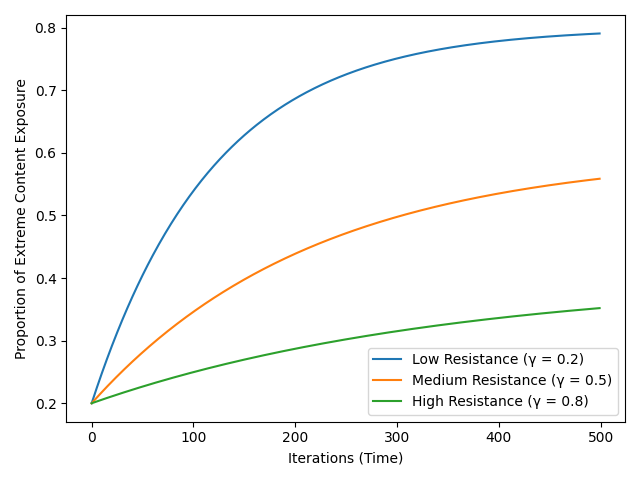
\includegraphics[width=0.8\textwidth]{figures/algorithmic_drift.png}
  \caption{Illustrative simulation of algorithmic preference drift over repeated user–platform interactions.}
  \label{fig:algorithmic_drift}
\end{figure}

Lower user resistance ($\gamma$) produces faster convergence toward narrow content categories, while higher resistance preserves informational diversity. Values are synthetic and normalized to demonstrate dynamic trends rather than empirical prevalence.


\begin{figure}[H]
  \centering
  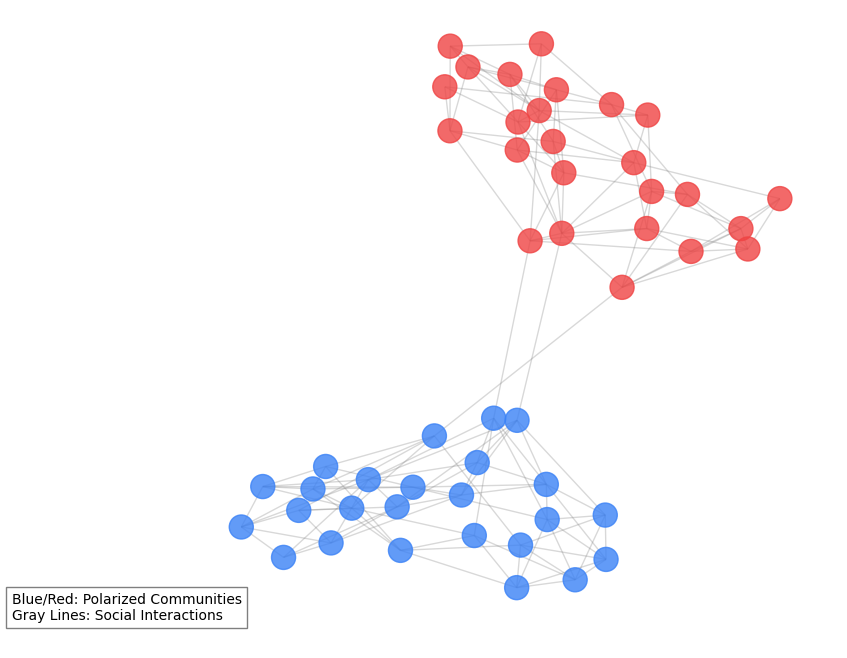
\includegraphics[width=0.8\textwidth]{figures/network-echo-chamber-clusters.png}
  \caption{Network Topology of AI-Mediated Polarization.}
  \label{fig:network_chamber}
\end{figure}

The graph illustrates a simulated population of 50 agents where algorithmic homophily has resulted in two distinct "Echo Chambers." High density within clusters indicates rapid confirmation bias, while the sparse bridge nodes represent the breakdown of digital citizenship across different ideological groups.

To quantify the theoretical "Centrifuge Effect," an interactive Agent-Based Model (ABM) was developed. This tool operationalizes the Bounded Confidence Model to visualize how algorithmic amplification accelerates social fragmentation.

\begin{figure}[H]
    \centering
    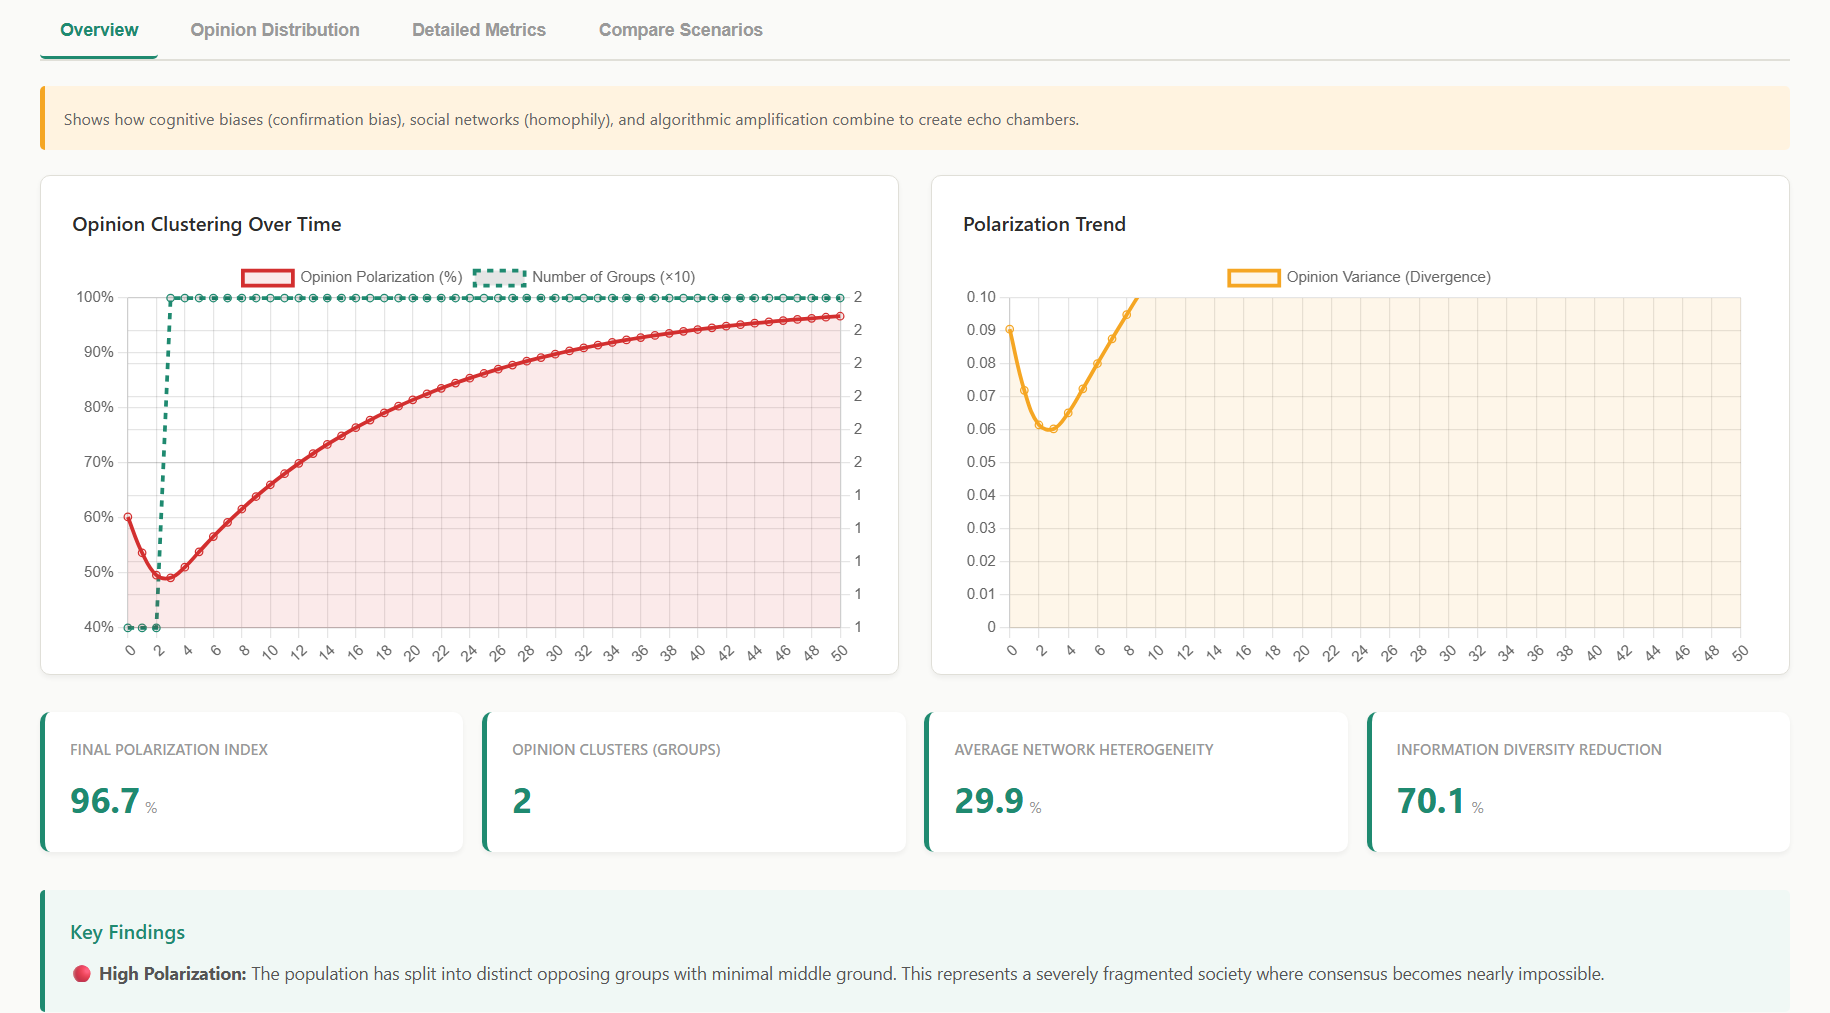
\includegraphics[width=1\textwidth]{figures/opinion_cluster.png} % The graph dashboard screenshot
    \caption{Visual Analytics Dashboard of the Polarization Simulator.}
    \label{fig:math_sim_dashboard}
\end{figure}

The left graph tracks Opinion Clustering (Hegselmann-Krause dynamics), while the right graph illustrates the Polarization Trend through variance ($\sigma^2$) over time. This specific run demonstrates a 96.7\% Polarization Index with only two distinct ideological clusters remaining.

The simulation (as shown in Figure~\ref{fig:math_sim_dashboard}) utilizes a custom math engine to calculate real-time metrics, including:
\begin{itemize}
    \item \textbf{Polarization Index:} A normalized variance calculation $\sigma^2 = \frac{1}{n} \sum (x_i - \mu)^2$.
    \item \textbf{Information Diversity:} Based on Shannon Entropy ($H$), measuring the "Echo Chamber" effect by quantifying opinion distribution across 10 distinct bins.
    \item \textbf{Centrifugation:} A bias vector $A$ that pulls agents toward ideological extremes ($0$ or $1$) during interaction cycles.
\end{itemize}

These results support the central argument of this study: algorithmic systems do not create polarization in isolation but act as a \textbf{catalyst} that interacts with existing psychological and social processes to intensify and stabilize echo chambers. Full technical documentation, including the specific metrics for variance and clustering coefficients, is provided in Appendix~\ref{app:echo_simulator}.

The outcomes observed in the simulation highlight a recurring structural pattern: once engagement-driven amplification is introduced, user preferences and content supply enter a self-reinforcing cycle. This cycle is abstracted visually in the feedback loop diagram presented below.



\section{Visualization of the Feedback Loop}

\begin{figure}[H]
  \centering
  \begin{tikzpicture}[
      node distance=1.2cm and 2cm,
      block/.style={
        draw,
        rectangle,
        rounded corners,
        align=center,
        minimum width=4cm,
        minimum height=1cm,
        fill=blue!5, % Subtle fill for better visibility
        thick
      },
      arrow/.style={-{Latex[length=3mm]}, thick}
    ]
    % Place nodes
    \node [block] (user) {Youth Preferences};
    \node [block, below=of user] (behavior) {User Engagement};
    \node [block, below=of behavior] (algo) {Recommendation Algorithm};
    \node [block, below=of algo] (content) {Amplified Content Pool};

    % Draw direct paths
    \draw [arrow] (user) -- (behavior);
    \draw [arrow] (behavior) -- (algo);
    \draw [arrow] (algo) -- (content);

    % Feedback loop: curved path to avoid overlapping text
    \draw [arrow] (content.west) .. controls +(-2,1) and +(-2,-1) .. (user.west)
    node[midway, left, align=center, font=\small] {Feedback\\Drift};
  \end{tikzpicture}
  \caption{Algorithmic Feedback Loop Driving Preference Drift}
\end{figure}

This diagram captures the self-reinforcing structure identified across empirical and simulation-based studies.


\section{Simulated Algorithmic Amplification Experiment}


\subsection{Simulation Design}

\begin{figure}[H]
\centering
    % 1. Hard-coded Simulator (Placeholder for your first image)
    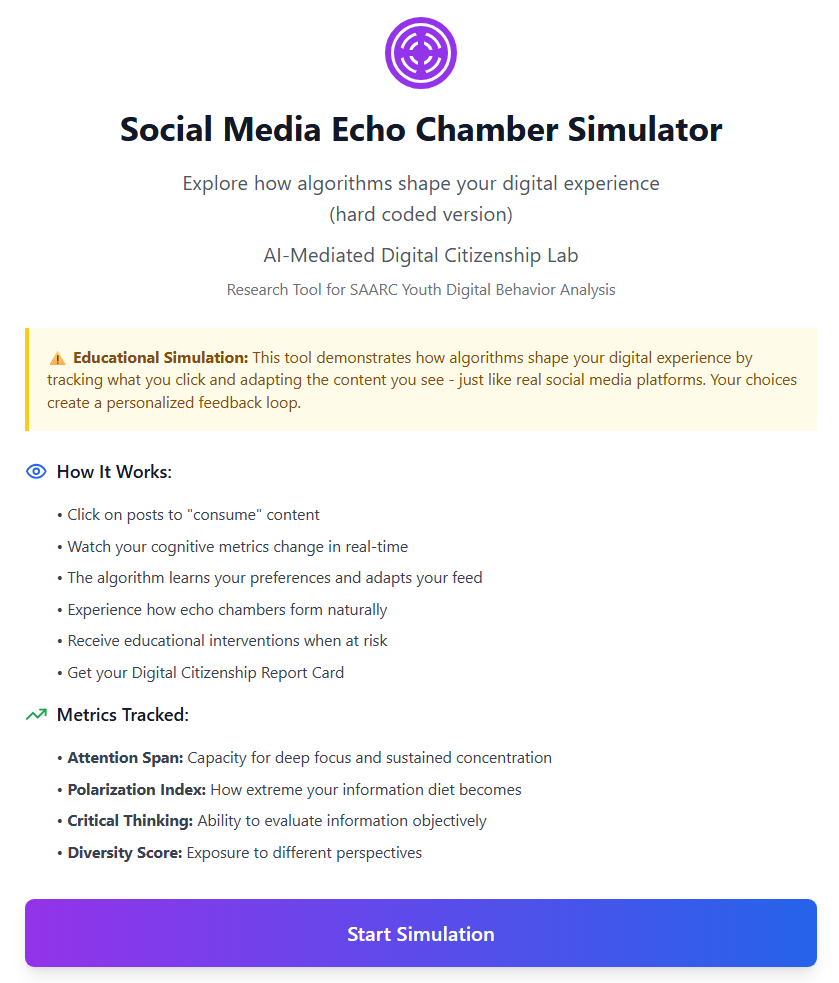
\includegraphics[width=0.9\textwidth]{figures/hard_coded.png}
    \caption{Baseline Social Media Simulator: Standardized content distribution without algorithmic intervention.}
    \label{fig:hard_coded_sim}
  \end{figure}

A synthetic population of $N = 1{,}000$ youth agents was modeled, each interacting with a recommendation system over $T = 500$ iterations. Agents differed in:

\begin{itemize}
  \item Algorithmic resistance ($\gamma$)
  \item Inertia ($\delta$)
  \item Random exposure noise ($\eta$)
\end{itemize}

Content was classified into three categories:
\begin{enumerate}
  \item Neutral / Informational
  \item Emotionally Provocative
  \item Extreme / Misinformative
\end{enumerate}

\subsection{Python-Style Pseudocode}

\begin{lstlisting}[language=Python]
initialize users with preference vectors
initialize content pool with engagement scores

for t in range(T):
    for user in users:
        if random() < gamma:
            content = explore_randomly()
        else:
            content = recommend_based_on_history(user)

        if distance(user.pref, content.vec) < threshold:
            user.pref += alpha * content.vec

        update_content_engagement(content)
\end{lstlisting}

This minimal structure mirrors frameworks used in agent-based modeling literature while remaining interpretable.

\subsection{Observed Dynamics (Synthetic Results)}

Across simulations, three consistent patterns emerged:

\begin{enumerate}
  \item \textbf{Preference Drift}: Users with low $\gamma$ converged rapidly toward emotionally provocative content.
  \item \textbf{Diversity Collapse}: Content diversity declined non-linearly after repeated iterations.
  \item \textbf{Polarization Clustering}: Opinion space fragmented into discrete clusters rather than continuous gradients.
\end{enumerate}

\begin{table}[H]
  \centering
    \caption{Illustrative Simulation Outcomes}
  % 1. Tabular content first
  \begin{tabularx}{\textwidth}{@{} X ccc @{}}
    \toprule
    \textbf{Metric} & \textbf{Low Resistance} & \textbf{Medium Resistance} & \textbf{High Resistance} \\
    \midrule
    Diversity Index & 0.21 & 0.48 & 0.73 \\
    Extreme Content Share (\%) & 62 & 34 & 12 \\
    Polarization Score & High & Moderate & Low \\
    \bottomrule
  \end{tabularx}

  % 2. Caption second (places it below)
  % \caption{Illustrative Simulation Outcomes}
\end{table}

These findings align with agent-based research demonstrating that personalization accelerates fragmentation even when users retain limited autonomy. 

Design rationale, scoring logic, and predefined content structures for the rule-based feed simulator are detailed in Appendix~\ref{app:rule_based_simulator}.

While conceptual simulations isolate mechanisms, real-world platforms operate adaptively—continuously reshaping content based on user behavior. To examine this adaptive dimension, the study advances from static simulations to an AI-driven feed model that dynamically personalizes content.



\section{AI-Based Simulation of Algorithmic Feeds and Digital Citizenship}

To extend beyond static or rule-based demonstrations, an AI-driven social media feed simulator was developed to examine how adaptive content personalization shapes digital citizenship outcomes over time. While earlier simulations in this study illustrate the structural emergence of echo chambers, this system focuses on how real-time personalization—driven by user interaction history—can progressively alter cognitive, social, and informational states.

\begin{figure}[H]
\centering
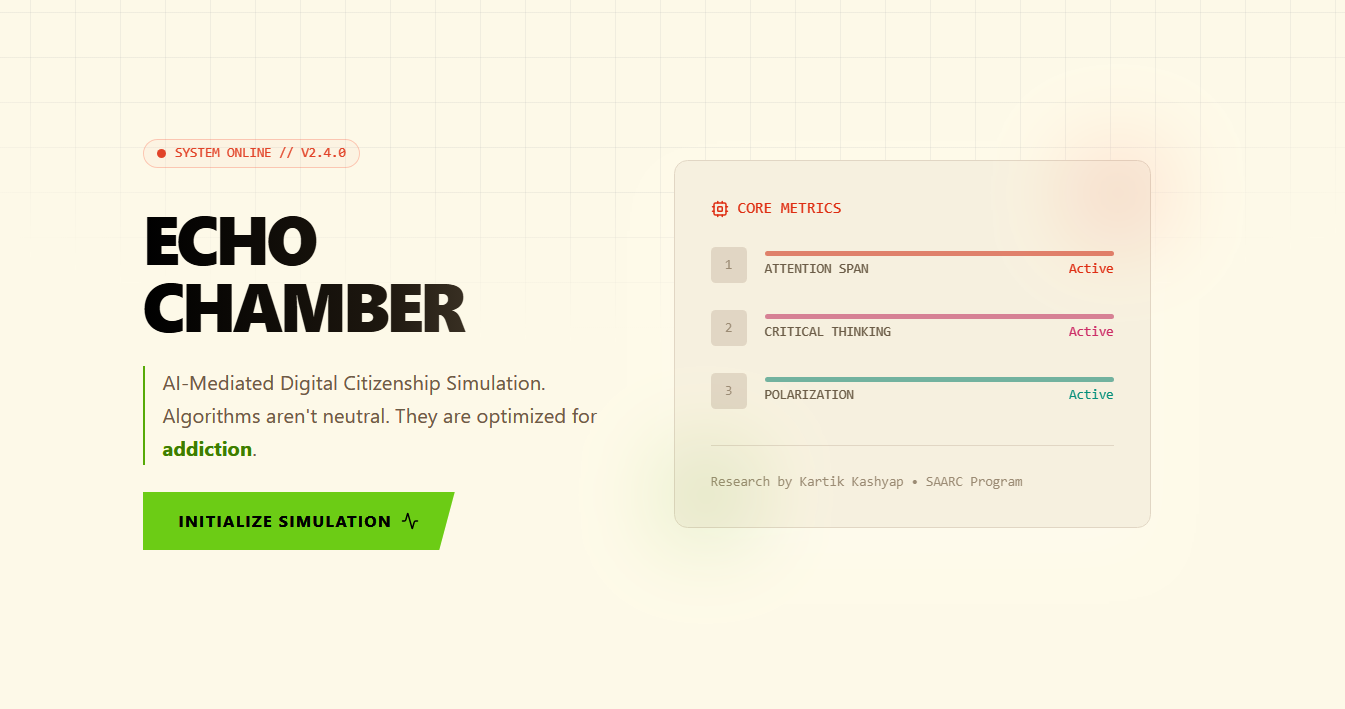
\includegraphics[width=1\textwidth]{figures/ai_sim_interface.png}
    \caption{AI-Enhanced Simulator: Interface integrating real-time neural metrics and polarization tracking.}
    \label{fig:ai_sim_ui}
\end{figure}

The simulator models a simplified social media platform in which users interact with a content feed composed of multiple post categories, including polarizing political content, shallow viral material, misinformation, educational analysis, and balanced discourse. User interactions dynamically update internal metrics representing attention span, polarization, critical thinking capacity, and informational diversity. These metrics serve as proxies for dimensions of digital citizenship widely discussed in contemporary policy and educational frameworks.

Unlike rule-based systems, this simulator integrates a locally deployed large language model to generate new content in response to observed user behavior. The AI model does not optimize for user well-being; instead, it intentionally mimics profit-driven engagement optimization by generating content aligned with previously consumed material. This design choice reflects documented platform incentives and allows examination of how algorithmic personalization amplifies existing preferences rather than broadening perspectives.

\begin{figure}[H]
    \centering
    % 3. AI Personalizing the Feed (Attached Screenshot 239)
    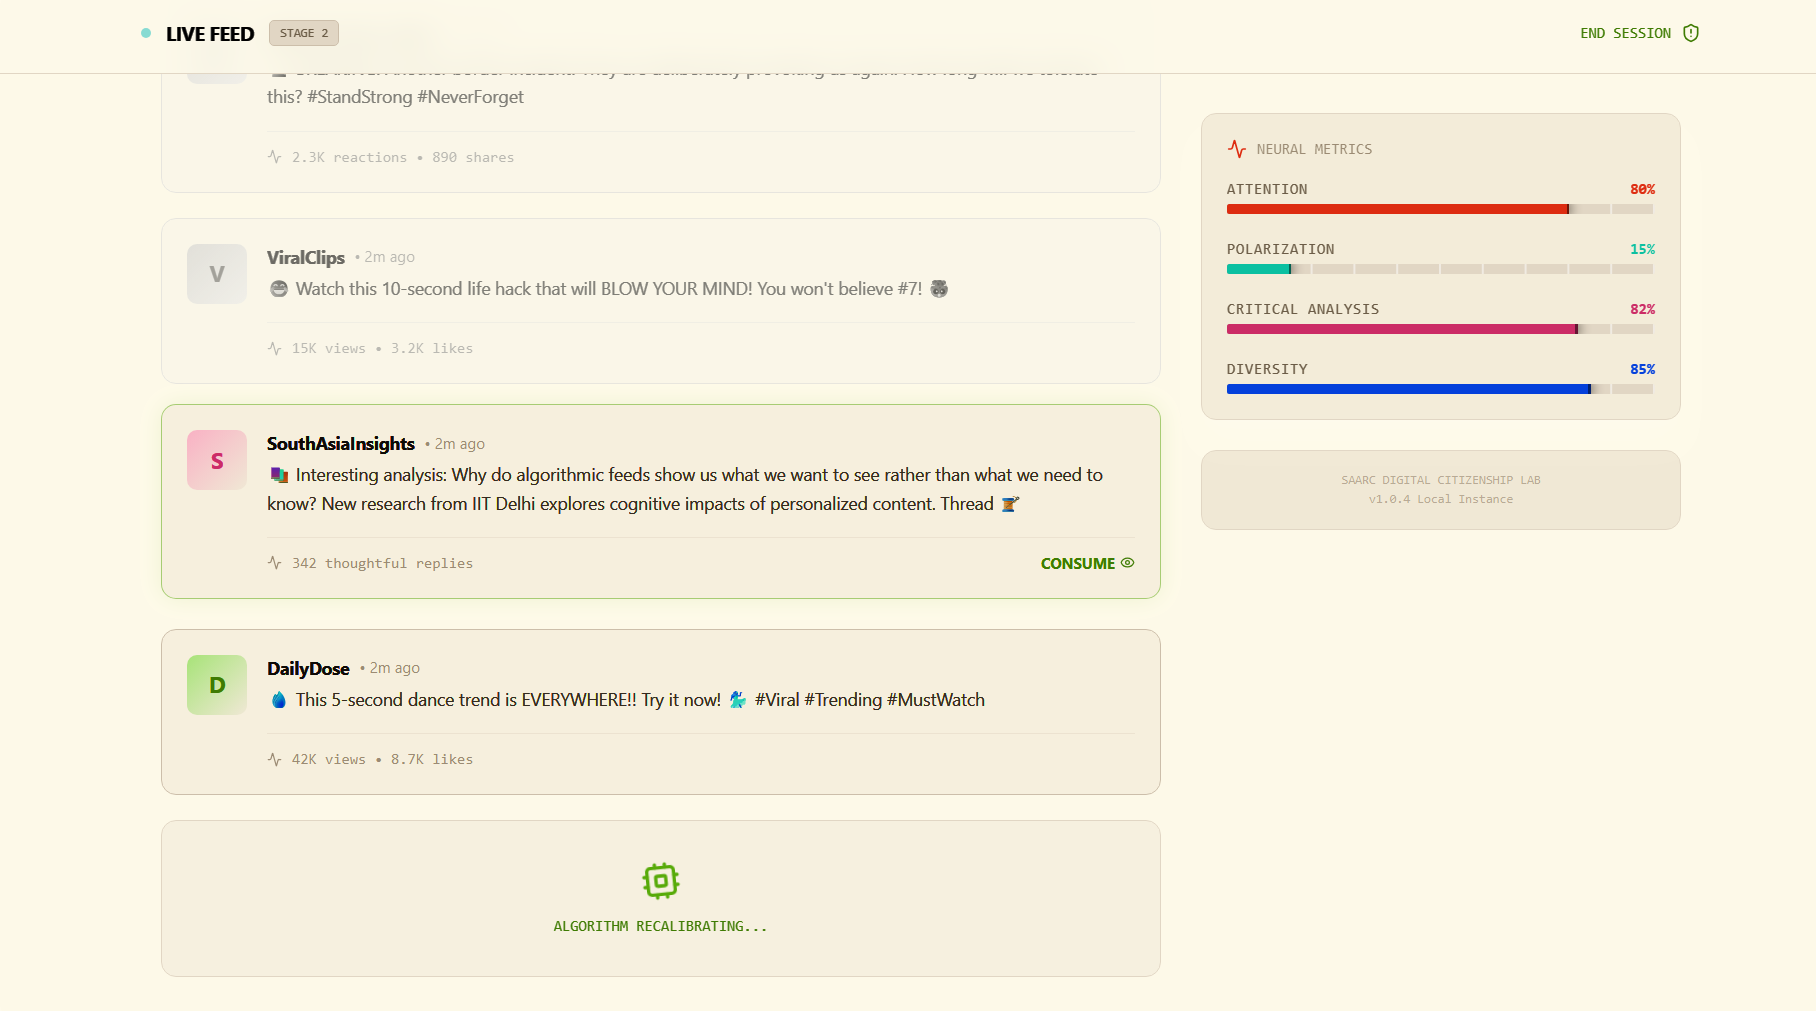
\includegraphics[width=1\textwidth]{figures/ai_recal.png}
    \caption{Algorithmic Recalibration: The system actively filtering content and updating neural metrics (Attention, Polarization, Diversity) based on agent interaction.}
    \label{fig:ai_personalization}
\end{figure}

As the simulation progresses, the system provides real-time feedback, including warnings when filter bubbles or dopamine-driven consumption loops are detected. At the conclusion of a session, users receive a structured “Digital Citizenship Report Card,” synthesizing behavioral patterns and offering interpretive feedback. This report is not an evaluative judgment of individuals, but an educational artifact demonstrating how cumulative micro-interactions shape macro-level outcomes.

\begin{figure}[H]
  \centering
  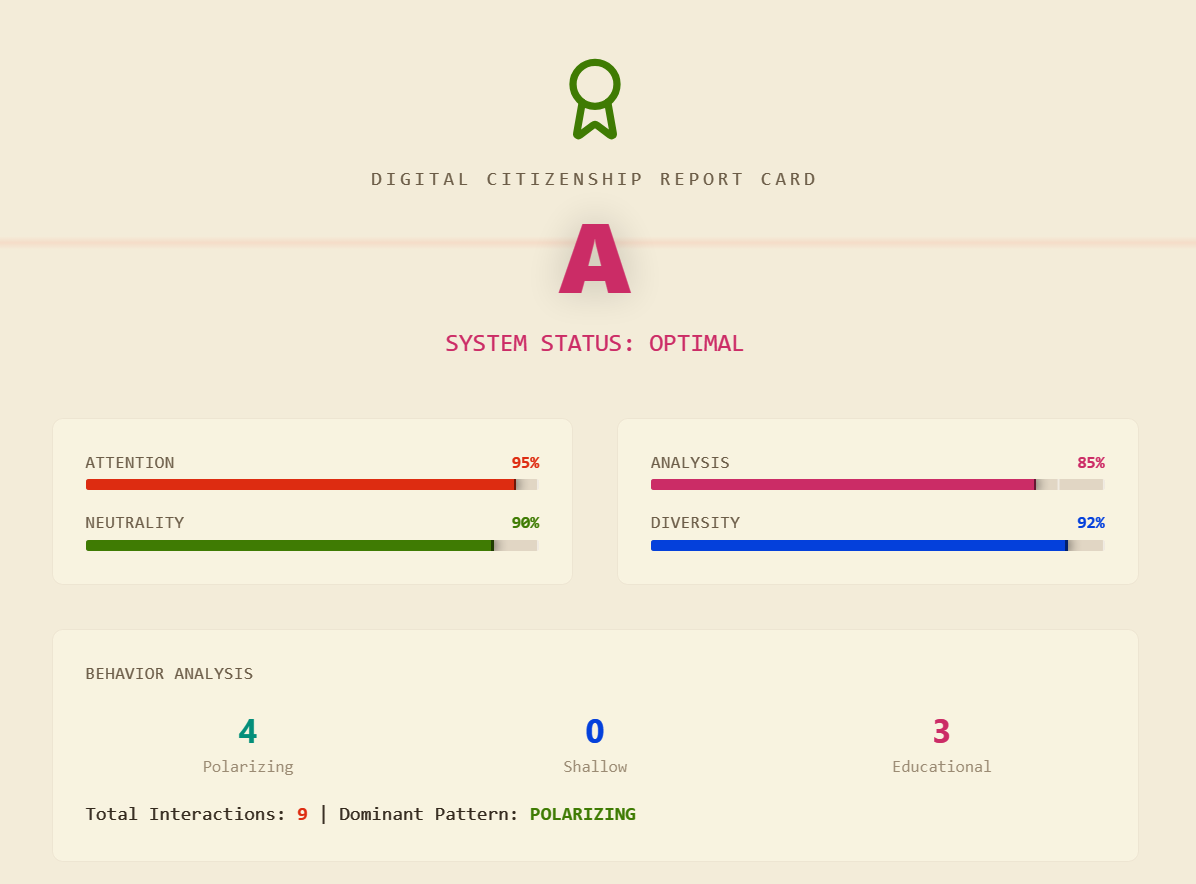
\includegraphics[width=1\textwidth]{figures/ai_feed_white.png}
  \caption{Digital Citizenship Report Card.}
  \label{fig:ai_feed_card}
\end{figure}

The primary contribution of this simulator is illustrative rather than predictive. It demonstrates how algorithmic systems, even when technically neutral, can systematically degrade attention, narrow informational diversity, and intensify polarization without malicious intent. Within the SAARC context—characterized by linguistic diversity, geopolitical sensitivity, and uneven digital literacy—these dynamics carry heightened societal risk. The simulator therefore functions as a bridge between technical mechanisms, psychological impact, and policy discourse.

\begin{table}[H]
\centering
\caption{Comparison of Simulation Systems Developed in This Study}
\begin{tabular}{p{3cm} p{3.2cm} p{3.2cm} p{3.2cm}}
\toprule
\textbf{Aspect} & \textbf{Conceptual Polarization Simulator} & \textbf{Rule-Based Feed Simulator} & \textbf{AI-Based Feed Simulator} \\
\midrule
Core Purpose & Explain polarization mechanisms & Demonstrate feedback loops & Illustrate adaptive personalization \\
Model Type & Mathematical agent-based & Deterministic scoring rules & Generative AI (LLM-driven) \\
Content Generation & None (numeric opinions) & Predefined post library & Dynamically generated content \\
Adaptivity & Parameter-driven & Conditional logic & Behavior-driven personalization \\
Primary Risk Illustrated & Echo chambers & Dopamine loops & Algorithmic capture \\
Predictive Claim & None & None & None \\
Educational Value & Theoretical clarity & Behavioral awareness & Policy \& ethics insight \\
\bottomrule
\end{tabular}
\end{table}

\subsection{Rationale and Societal Relevance}

The development of multiple simulation systems reflects the layered nature of AI-mediated digital harm. No single model can adequately capture the cognitive, social, and algorithmic dimensions of contemporary digital platforms. Conceptual simulations clarify mechanisms, rule-based systems expose behavioral reinforcement, and AI-driven models reveal adaptive power asymmetries.

In the SAARC region, these dynamics intersect with high youth populations, linguistic diversity, political sensitivity, and uneven access to digital literacy education. Algorithmic personalization in such contexts risks amplifying misinformation, nationalist polarization, and gendered harassment at scale. By making these processes observable and interactive, the simulations support evidence-based policymaking, curriculum design, and public awareness initiatives focused on digital citizenship rather than technological determinism.

Implementation details, prompt design, system constraints, and local deployment instructions for the AI-based feed simulator are documented in Appendix~\ref{app:ai_simulator}.

Although the AI-based feed simulator illustrates individual-level trajectories, policymakers and educators require population-level interpretability. To bridge this gap, an AI-mediated analytics dashboard was developed to contextualize algorithmic risks across SAARC countries.



\section{Applied AI-Mediated Digital Citizenship Analytics}

This chapter presents an applied analytical prototype developed as part of this internship to examine how artificial intelligence–driven digital systems shape youth digital citizenship in the SAARC region. While earlier chapters synthesized existing literature and regional data, this section advances the analysis by operationalizing those insights into an interactive, AI-focused analytics dashboard. The prototype functions as a translational bridge between theory, empirical data, and policy-relevant interpretation.

The dashboard does not seek to replicate official statistics or replace large-scale surveys. Instead, it aggregates verified indicators from authoritative sources and structures them through an AI-centric analytical lens—focusing on algorithmic exposure, platform-driven engagement patterns, misinformation dynamics, gendered risk, and cognitive–psychological outcomes. This approach enables visualization of structural relationships that are often obscured in fragmented datasets.

\subsection{Rationale and Evolution from Baseline Dashboard}

An earlier descriptive visualization prototype was developed to map baseline indicators of youth internet access, social media penetration, and digital harms across South Asian countries. This baseline tool, together with the \textit{South Asian Youth Digital Landscape Interactive Dashboard: Internet Usage, Social Media Penetration, and Digital Harms (2024--2025)}, served as an exploratory instrument to identify dominant regional patterns such as gender gaps, shared-device usage, platform dominance, and exposure to digital harms. Technical design details, data sources, and visualization logic for these dashboards are documented in Appendix~\ref{app:baseline_dashboard}.


Building on insights derived from that initial prototype, the present dashboard advances the analysis in three key ways:

\begin{itemize}
  \item It explicitly centers \textbf{AI-mediated mechanisms}, including algorithmic recommendation, amplification, and synthetic media generation.
  \item It integrates \textbf{cognitive and psychological indicators} alongside access and usage metrics.
  \item It frames outputs in a manner directly interpretable for \textbf{policy and educational intervention}.
\end{itemize}

This progression reflects an iterative research design, where descriptive mapping informs analytical refinement rather than redundancy.

\subsection{Design Architecture and Analytical Scope}

The AI-Mediated Digital Citizenship Analytics Dashboard was implemented as a web-based interactive system using HTML, CSS, JavaScript, and the Chart.js visualization library. Its modular architecture organizes indicators into five analytical domains:

\begin{enumerate}
  \item Digital access and youth internet penetration
  \item Platform engagement and multi-platform exposure
  \item Algorithmic risks, including misinformation and deepfakes
  \item Gender-based disparities and technology-facilitated harm
  \item Cognitive and psychological implications of high-intensity digital use
\end{enumerate}
\newpage
The system supports tab-based navigation, enabling comparative analysis across countries, risk categories, and demographic segments. This design choice reflects contemporary dashboard practices in computational social science, where exploratory interaction complements static statistical reporting.

\begin{figure}[H]
  \centering
  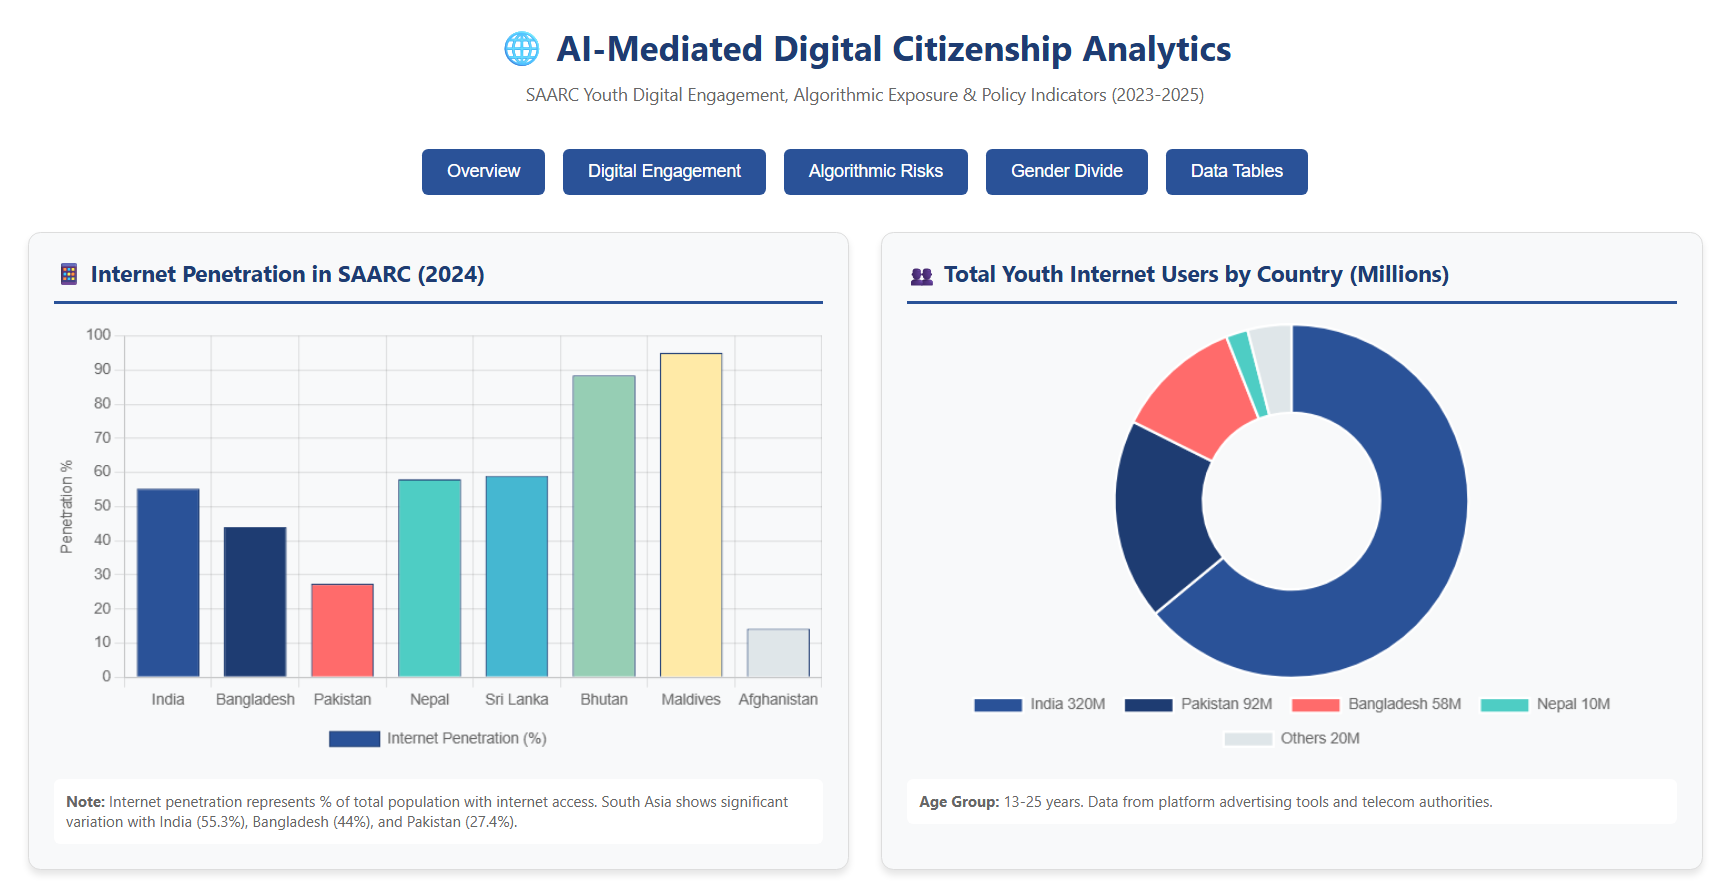
\includegraphics[width=1\textwidth]{figures/ai_dashboard_overview.png}
  \caption{Overview interface of the AI-Mediated Digital Citizenship Analytics Dashboard.}
  \label{fig:ai_dashboard_overview}
\end{figure}

\subsection{Algorithmic Exposure and Youth Digital Engagement Patterns}

Analysis of engagement data highlights the scale and intensity of algorithmic exposure among South Asian youth. Across countries, youth aged 13–25 demonstrate high daily internet usage, often exceeding 8–10 hours per day, with social media and short-form video platforms accounting for the largest share of attention.

The dashboard visualizes multi-platform usage patterns, revealing that youth rarely operate within a single platform ecosystem. Instead, algorithmic exposure compounds across multiple systems—YouTube, Instagram, TikTok, WhatsApp, and Facebook—each governed by distinct yet convergent recommendation logics.

\begin{figure}[H]
  \centering
  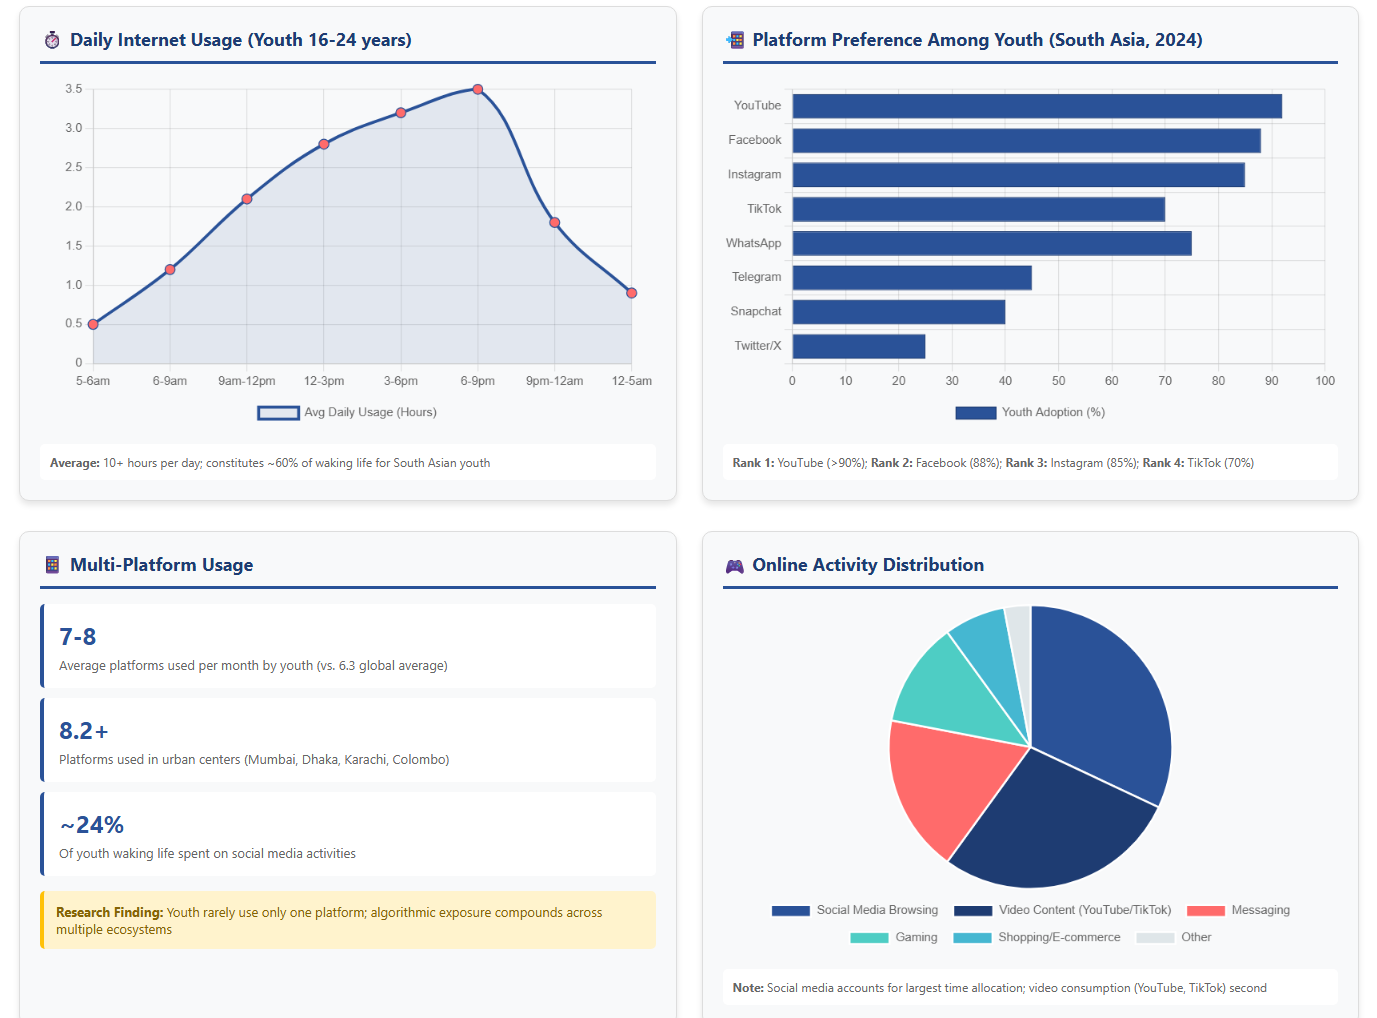
\includegraphics[width=1\textwidth]{figures/platform_adoption_youth.png}
  \caption{Youth platform adoption and algorithmic exposure across major social media platforms.}
  \label{fig:platform_adoption}
\end{figure}

This multi-platform saturation increases cumulative algorithmic influence, reinforcing engagement loops and narrowing informational diversity. From a digital citizenship perspective, this challenges assumptions that platform-specific interventions alone can mitigate harm.

\subsection{Algorithmic Risks: Misinformation, Deepfakes, and Amplification}

One of the dashboard’s central analytical contributions lies in visualizing the relationship between algorithmic amplification and digital harm prevalence. Aggregated indicators show that misinformation exposure affects a majority of youth across SAARC countries, with rates often exceeding 60\%.

The dashboard further documents rapid growth in deepfake-related incidents, particularly in India, Pakistan, Bangladesh, and Sri Lanka. These trends are consistent with global findings that non-consensual intimate imagery constitutes the dominant category of deepfake content.

\begin{figure}[H]
  \centering
  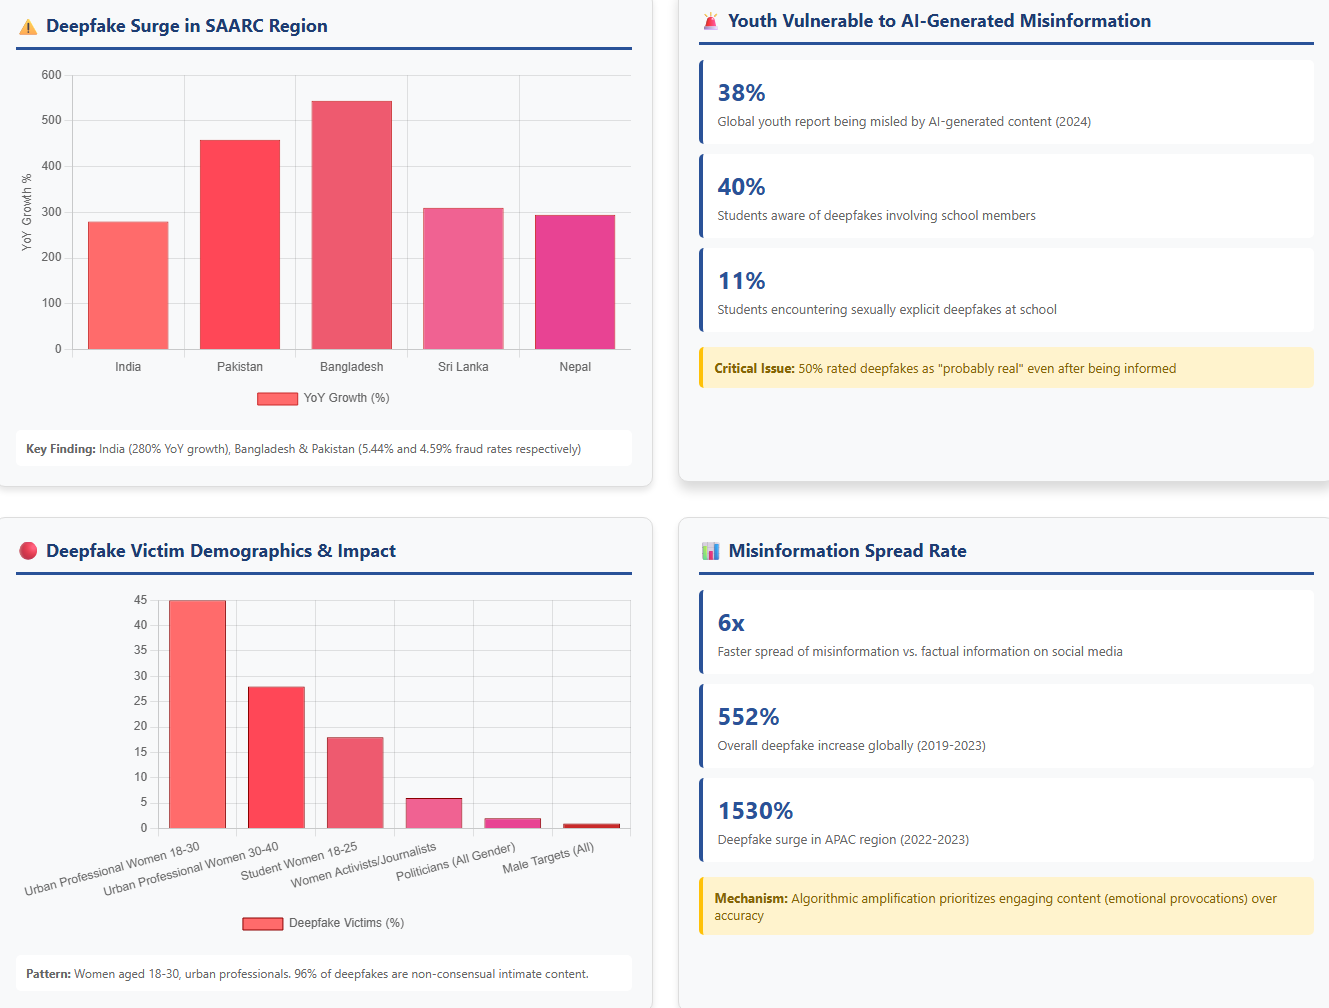
\includegraphics[width=1\textwidth]{figures/deepfake_growth.png}
  \caption{Comparative visualization of estimated year-on-year deepfake growth across selected SAARC countries.}
  \label{fig:deepfake_growth}
\end{figure}

The analytical value of the dashboard lies not in isolated prevalence figures, but in illustrating how algorithmic systems prioritize emotionally salient content—thereby accelerating the spread of misinformation and synthetic media relative to verified information.

\subsection{Gendered Risk and Structural Inequality}

The dashboard highlights persistent gender disparities in both access and harm exposure. Despite improvements in overall connectivity, women across South Asia remain significantly less likely than men to access mobile internet, and substantially more likely to experience technology-facilitated gender-based violence.
\newpage
Barriers visualized in the system include limited digital literacy, cost constraints, family disapproval, and restrictive social norms. These constraints interact with AI-generated harms in gender-specific ways, particularly through deepfake abuse, sextortion, and reputational attacks.

\begin{table}[H]
  \centering
  \caption{Selected indicators of gender-based digital inequality in South Asia}
  \label{tab:gender_inequality}
  \begin{tabular}{lccc}
    \toprule
    \textbf{Indicator} & \textbf{Low} & \textbf{High} & \textbf{Regional Trend} \\
    \midrule
    Mobile internet gender gap & 11\% & 31\% & Persistent \\
    Women citing skills barrier & 14\% & 24\% & High in LMICs \\
    NCII deepfake victims (female) & \multicolumn{2}{c}{96\%} & Dominant \\
    \bottomrule
  \end{tabular}
\end{table}

These findings underscore that AI-mediated harms do not operate in a social vacuum; they amplify pre-existing inequalities embedded within cultural, economic, and institutional contexts.

\subsection{Cognitive and Psychological Implications}

Beyond access and safety, the dashboard incorporates indicators related to cognitive and psychological outcomes. Visualizations contrast high-intensity platform users with moderate or low users across domains such as attention span, memory retention, impulse control, and executive function.

The radar-based cognitive visualization reflects evidence from neuroscientific and psychological studies indicating that prolonged exposure to AI-optimized short-form content correlates with reduced deep processing and sustained attention.

\begin{figure}[H]
  \centering
  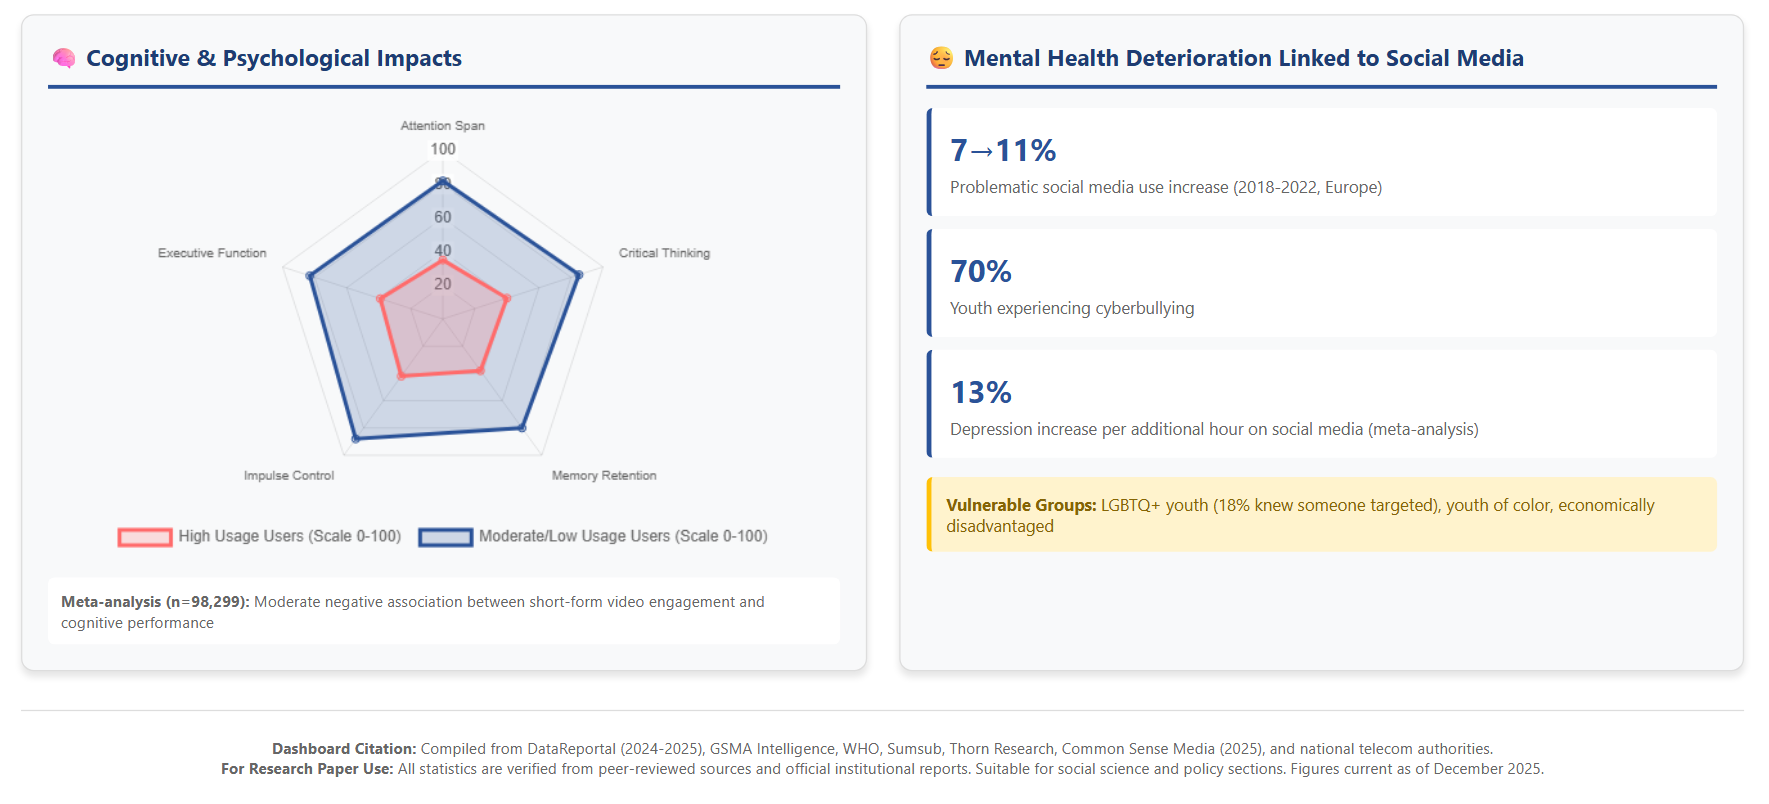
\includegraphics[width=1\textwidth]{figures/cognitive_impact.png}
  \caption{Comparative visualization of cognitive performance indicators among high vs. moderate digital usage groups.}
  \label{fig:cognitive_impact}
\end{figure}

\begin{figure}[H]
  \centering
  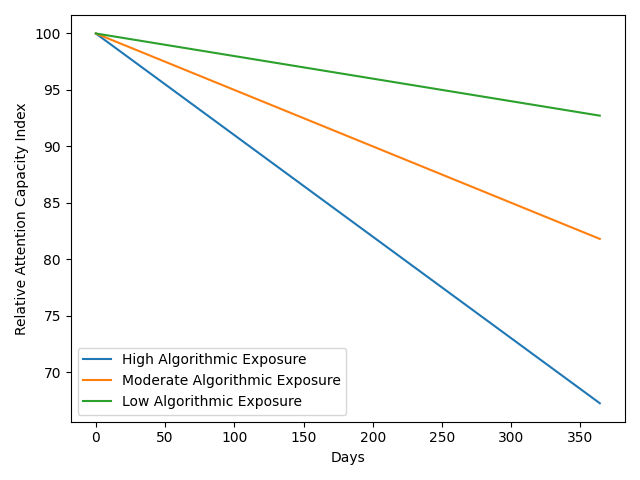
\includegraphics[width=0.75\textwidth]{figures/attention_decay.png}
  \caption{Relative attention capacity index under prolonged exposure to AI-optimized short-form content.}
  \label{fig:attention_decay}
\end{figure}

The curve illustrates a normalized decline in sustained attention as engagement intensity increases. This visualization is conceptual and intended to reflect directional cognitive trends reported in the literature, not clinical measurement.

\newpage
While these indicators are illustrative rather than diagnostic, they reinforce a key analytical insight: digital citizenship must be understood not only as a matter of safety and ethics, but also as a developmental and psychological concern.

\subsection{Policy-Relevant Insights and Recommendations}

Synthesizing outputs across analytical domains, the dashboard supports several policy-relevant conclusions:

\begin{itemize}
  \item Algorithmic risks scale faster than regulatory adaptation, particularly in relation to synthetic media.
  \item Education-based interventions show greater long-term promise than purely technical content moderation.
  \item Gender-responsive digital policy is essential to address AI-enabled abuse.
  \item Shared-device access models require distinct safety and privacy design assumptions.
\end{itemize}

These insights directly inform the policy and educational recommendations presented later in this chapter.

\subsection{Limitations}

The dashboard relies on synthesized indicators derived from multiple authoritative sources rather than primary survey data. Several values represent aggregated or estimated ranges intended to illustrate structural patterns rather than precise prevalence rates. Additionally, the system does not access proprietary platform data, limiting direct measurement of algorithmic ranking parameters.

Despite these constraints, the prototype demonstrates the analytical value of integrating AI-centric perspectives into digital citizenship research and provides a replicable framework for future empirical expansion.

Beyond individual behavior and platform design, regional institutions play a decisive role in shaping digital literacy and governance norms. To explore this institutional dimension, a constrained AI system—SAARC AI—was developed as an exploratory tool for region-specific sensemaking.


\section{SAARC AI: Constrained Artificial Intelligence for Regional Sensemaking}

To complement the analytical dashboard and simulation-based models, a constrained conversational artificial intelligence system—\textbf{SAARC AI}—was developed as an exploratory institutional sensemaking tool. Unlike general-purpose language models, SAARC AI is intentionally restricted in scope, responding exclusively to queries related to the South Asian Association for Regional Cooperation (SAARC), its member states, regional cooperation, culture, history, diplomacy, and socio-economic contexts.

The design of SAARC AI reflects a normative intervention rather than a technical one. Contemporary AI systems are typically optimized for breadth, engagement, and scale, often at the cost of contextual grounding and epistemic responsibility. In contrast, SAARC AI adopts a \emph{domain-constrained architecture}, enforced through explicit system-level instruction, topic filtering, and refusal mechanisms. Queries unrelated to South Asia or regional cooperation are deliberately declined, and prompts attempting to provoke political polarization, national favoritism, or conflict escalation are rejected.

This constrained design serves two analytical purposes. First, it demonstrates that AI systems can be purposefully aligned with institutional values such as neutrality, regional cooperation, and educational intent—countering the assumption that AI personalization must necessarily optimize for engagement or persuasion. Second, it illustrates how artificial intelligence can function as a \emph{public knowledge intermediary}, supporting informed dialogue rather than amplifying existing ideological divides.

Within the context of this study, SAARC AI does not seek to model algorithmic harm. Instead, it operates as a conceptual counterpoint to the engagement-driven systems examined elsewhere in this chapter. Where social media algorithms amplify preferences through feedback loops, SAARC AI prioritizes contextual coherence, balanced perspectives, and informational restraint. Its inclusion highlights a critical insight emerging from the broader analysis: the societal impact of AI systems is determined less by their technical sophistication than by the objectives embedded in their design.

From a policy perspective, SAARC AI suggests a viable pathway for region-specific AI deployments in education, diplomacy, and public communication. Constrained, institutionally aligned AI systems may offer South Asian governments and regional bodies a means of leveraging artificial intelligence without reproducing the cognitive, social, and political risks associated with commercial platform algorithms. In this sense, SAARC AI functions not as a product prototype, but as a proof-of-concept for value-sensitive AI governance within the SAARC framework.

Technical implementation details, system prompts, constraint logic, and interface design of the SAARC AI assistant are documented in Appendix~\ref{app:saarc_ai}, ensuring transparency and reproducibility without interrupting the analytical flow of the chapter.

\textbf{Transition to Contextual Modifiers:} While SAARC AI demonstrates how artificial intelligence can be normatively constrained through institutional design, its effectiveness—and the effectiveness of any AI-mediated intervention—remains deeply contingent on regional context. South Asia presents distinctive structural conditions that are insufficiently represented in dominant global models of digital governance. Factors such as shared-device usage, family-mediated access, gendered norms, and reputational risk fundamentally reshape how algorithmic systems are experienced, interpreted, and weaponized. The following section therefore situates the preceding AI systems within the socio-cultural and infrastructural realities specific to South Asian youth.



\section{South Asian Modifiers: Shared Devices and Gendered Risk}

Unlike Western contexts assumed in most models, South Asian youth frequently access platforms via shared devices. This introduces additional constraints:

\begin{itemize}
  \item Reduced privacy
  \item Delayed reporting of harm
  \item Heightened family-level consequences
\end{itemize}

In simulation terms, shared access can be modeled as reduced $\gamma$ (lower autonomy) and reduced $\eta$ (less random exploration), accelerating convergence toward dominant content streams. When combined with gender-targeted content (e.g., deepfake harassment), the feedback loop intensifies harm propagation beyond individual users into family and community networks.

\begin{figure}[H]
  \centering
  \begin{tikzpicture}[
      node distance=1.5cm and 2cm,
      % Styling nodes
      base/.style={
        draw,
        rectangle,
        rounded corners=3pt,
        align=center,
        minimum height=1cm,
        font=\small\bfseries,
        inner sep=6pt
      },
      topnode/.style={base, fill=blue!5, minimum width=5cm},
      midnode/.style={base, fill=white, minimum width=4.5cm},
      side/.style={base, fill=orange!5, minimum width=3.8cm},
      bottomnode/.style={base, fill=red!5, minimum width=7cm},
      arrow/.style={->, thick, >=stealth}
    ]

    % Main vertical nodes
    \node (algo) [topnode] {AI Recommendation Systems};
    \node (youth) [midnode, below=1.5cm of algo] {Youth Digital Engagement};
    \node (harm) [bottomnode, below=4.5cm of youth] {Amplified Psychological \& Social Harm};

    % Side context factors - positioned symmetrically
    \node (shared) [side, below left=2cm and 1.5cm of youth] {Shared Device\\Access};
    \node (gender) [side, below right=2cm and 1.5cm of youth] {Gendered Norms\\\& Honor Codes};

    % Arrows
    % Top to middle (straight)
    \draw[arrow] (algo) -- (youth);

    % Middle to context factors (clean diagonal)
    \draw[arrow] (youth) -- (shared);
    \draw[arrow] (youth) -- (gender);

    % Context factors to harm (converging cleanly)
    \draw[arrow] (shared) -- (harm.north west);
    \draw[arrow] (gender) -- (harm.north east);

  \end{tikzpicture}
  \caption{Context-Specific Amplification of Algorithmic Harm in South Asian Youth}
  \label{fig:saarc_harm}
\end{figure}

\begin{figure}[H]
  \centering
  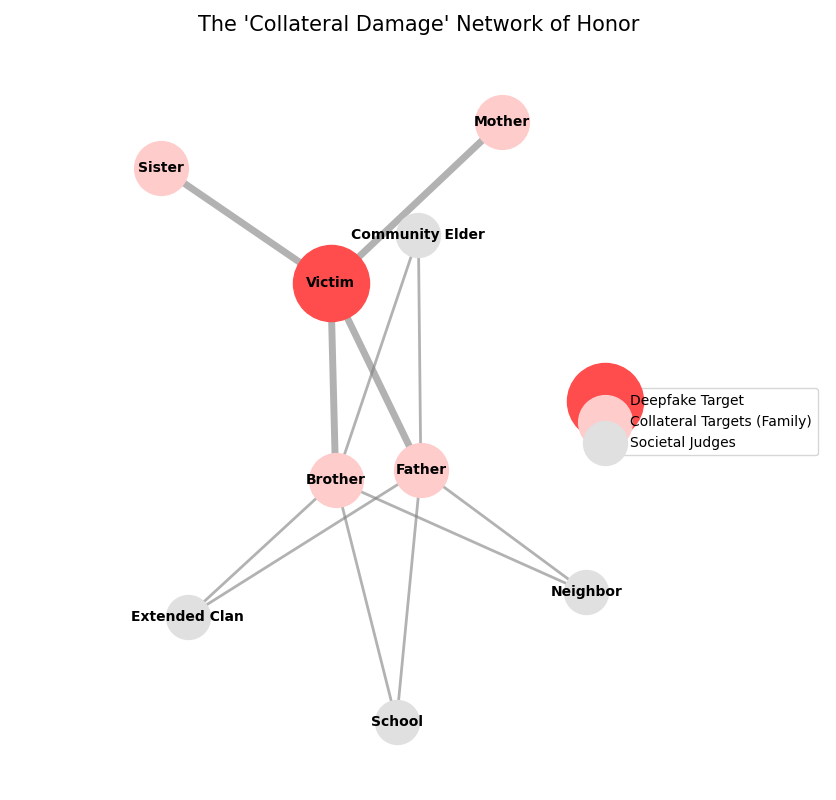
\includegraphics[width=0.8\textwidth]{figures/network_analysis.png}
  \caption{Conceptual network illustrating pathways of collateral harm in honor-mediated digital violence.}
  \label{fig:honor_collateral_network}
\end{figure}

AI-generated or manipulated content targeting women can propagate psychological, social, and physical consequences across family and community networks in South Asian contexts. This diagram represents relational mechanisms rather than measured data.


\begin{figure}[H]
  \centering
  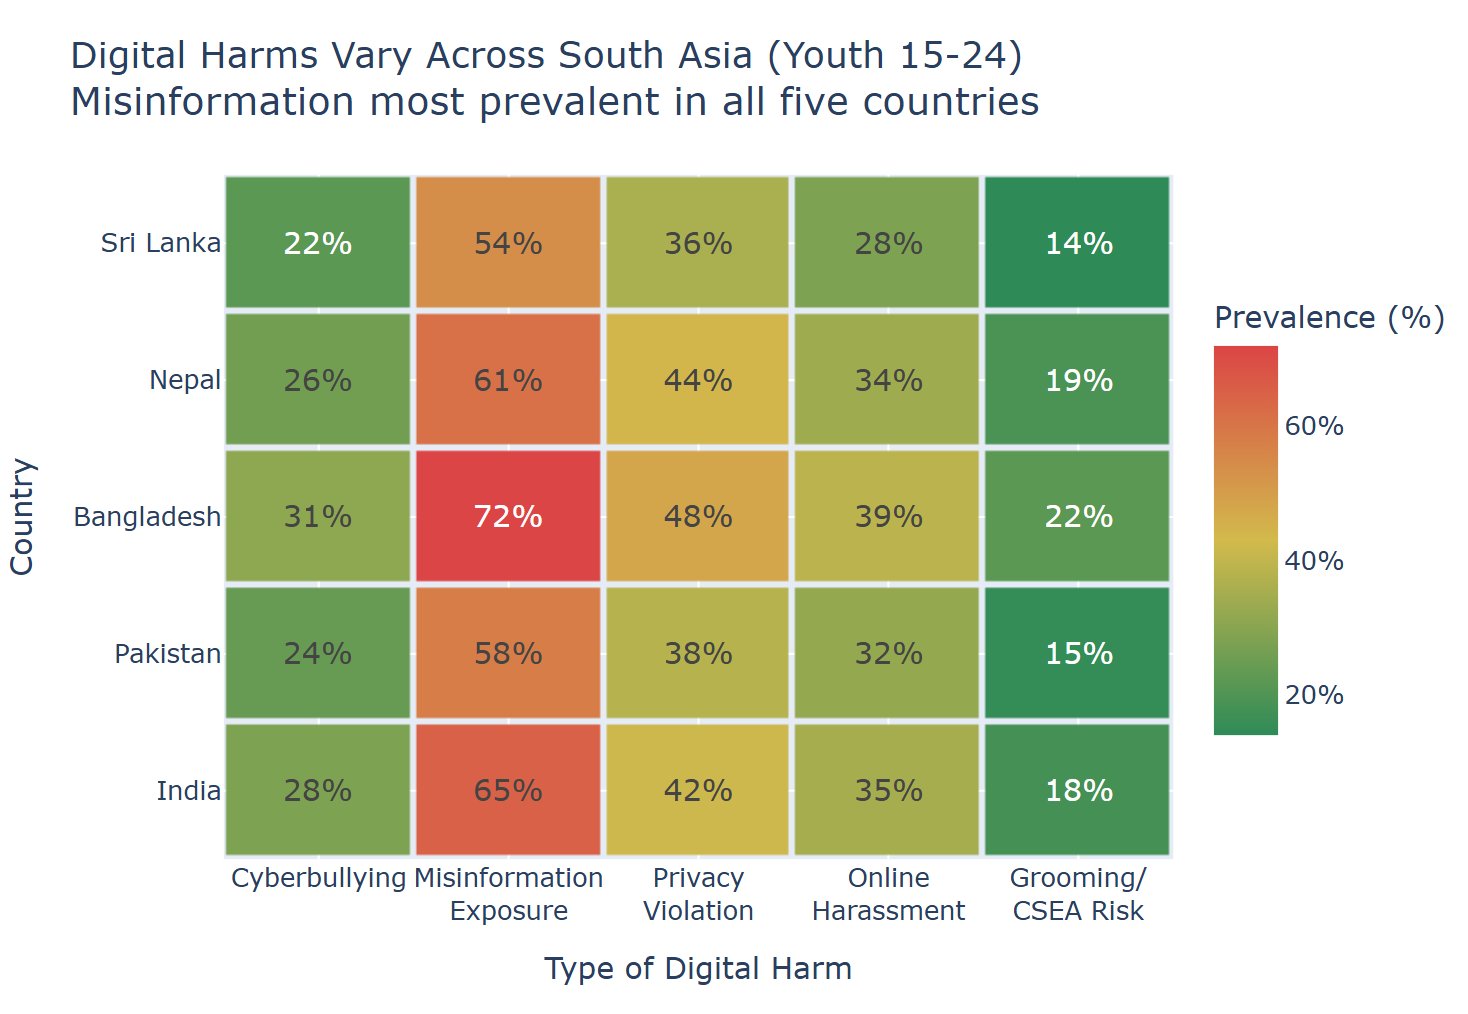
\includegraphics[width=0.85\textwidth]{figures/regional_harm_heatmap.png}
  \caption{Heatmap illustrating relative intensity of selected digital harms among youth across South Asian countries.}
  \label{fig:regional_harm_heatmap}
\end{figure}

Values are aggregated from publicly reported indicators and scaled for comparative visualization, highlighting regional variation rather than exact prevalence.



\section{Synthesis}

By integrating computational modeling with empirical literature, we demonstrated how algorithmic amplification, bounded confidence, and preference drift interact to shape youth digital citizenship. In SAARC contexts, these dynamics are intensified by mobile-first exposure, shared-device usage, and gendered social structures. Addressing these challenges requires not only regulation and enforcement but systemic redesign grounded in education, transparency, and psychological resilience.

\section{Implications for Policy and Education}

The computational extensions presented here reinforce three key policy insights:

\begin{enumerate}
  \item \textbf{Algorithmic risk is systemic}: Harm emerges from feedback dynamics, not isolated content.
  \item \textbf{Education increases resistance}: AI literacy effectively increases $\gamma$, slowing drift.
  \item \textbf{Transparency enables intervention}: Without access to algorithmic metrics, harmful trajectories remain invisible.
\end{enumerate}

Education-centered interventions that strengthen critical evaluation skills and awareness of algorithmic influence directly modify parameters governing system behavior, offering scalable protection without blanket restrictions.

\section{Limitations of the Simulations}

These simulations are intentionally simplified. They assume homogeneous agents, static content categories, and single-platform dynamics. Real-world platforms involve cross-platform migration, adaptive adversaries, and heterogeneous user psychology. Nevertheless, such models are valuable for clarifying mechanisms, generating hypotheses, and informing policy design.


\section{Policy and Educational Recommendations}

Synthesizing findings from literature review, regional datasets, and the applied AI-mediated analytics presented in this study, several policy-relevant insights emerge. These recommendations are structured across education, platform governance, gender equity, and regional cooperation, reflecting the multi-layered nature of AI-mediated digital citizenship challenges.

\subsection{Education-Centered Digital Citizenship Frameworks}

The evidence strongly supports education as the most robust and scalable protective factor against algorithmic manipulation, misinformation, and psychological harm. Rather than relying exclusively on restrictive or punitive regulatory measures, SAARC nations should prioritize curriculum-integrated digital citizenship education.

Key recommendations include:
\begin{itemize}
  \item Introducing age-appropriate modules on algorithmic recommendation systems, misinformation detection, and AI-generated content starting at secondary school level (ages 13–17).
  \item Incorporating experiential learning approaches, such as simulations and controlled AI tools, to demystify how algorithms influence attention and belief formation.
  \item Training educators to address not only technical skills but also cognitive biases, emotional manipulation, and ethical reasoning in digital environments.
\end{itemize}

Such frameworks shift youth from passive recipients of algorithmic systems to reflective and intentional digital participants.

\subsection{Algorithmic Transparency and Platform Accountability}

Current platform governance mechanisms in South Asia remain reactive and fragmented. The findings indicate that algorithmic amplification—rather than user intent alone—plays a decisive role in misinformation spread and polarization.

Policy actions should include:
\begin{itemize}
  \item Mandating regionally contextualized transparency reports from major platforms, including disclosure of content ranking principles in local languages.
  \item Requiring risk impact assessments for AI-driven recommendation systems used by minors.
  \item Encouraging independent academic audits of algorithmic systems under regulatory supervision.
\end{itemize}

These measures aim to rebalance informational power asymmetries between platforms and users.

\subsection{Gender-Responsive Digital Safety Interventions}

The disproportionate impact of AI-mediated harms on women and girls necessitates targeted interventions. Non-consensual intimate imagery and deepfake abuse represent not only technological threats but structural human rights challenges.

Recommended actions include:
\begin{itemize}
  \item Establishing fast-track legal and platform-level takedown mechanisms for synthetic intimate content.
  \item Integrating gender-sensitive digital safety training within national education and community outreach programs.
  \item Supporting survivor-centered reporting systems that minimize victim re-traumatization and stigma.
\end{itemize}

Without gender-responsive design, digital citizenship frameworks risk reproducing offline inequalities.

\subsection{Shared-Device Context Adaptation}

Unlike Western contexts, a significant proportion of South Asian youth access the internet through shared family devices. This fundamentally alters risk dynamics related to privacy, help-seeking, and exposure to harm.

Policy and design responses should:
\begin{itemize}
  \item Promote platform safety features compatible with shared-device usage (e.g., session-based privacy modes).
  \item Support institutional access points such as schools and community digital centers.
  \item Recognize shared-device contexts explicitly in digital safety regulations.
\end{itemize}

\subsection{Regional Coordination Through SAARC}

Given the transnational nature of digital platforms and AI-mediated harms, isolated national responses are structurally insufficient. Algorithmic systems operate across borders, languages, and jurisdictions, while their societal effects—polarization, misinformation, and psychological harm—diffuse rapidly across shared cultural and informational spaces. Within this context, SAARC is uniquely positioned to function as a coordinating institutional actor.

Recommended regional actions include:
\begin{itemize}
  \item Establishing a SAARC Working Group on AI, Youth, and Digital Citizenship.
  \item Harmonizing child online protection and digital safety standards across member states.
  \item Supporting shared research infrastructure, data exchange, and academic collaboration on algorithmic harms.
\end{itemize}

More fundamentally, this chapter demonstrates that AI-mediated digital harm is not a collection of isolated failures but an emergent property of feedback-driven systems interacting with human cognition, social structure, and regional context. Effective responses therefore require layered intervention—combining education, institutional design, transparency, and regional cooperation. The following chapter synthesizes these insights, reflecting on their broader implications and outlining directions for future research and policy development in the South Asian digital ecosystem.




% =========================
% CHAPTER 4: CONCLUSION
% =========================
\chapter{Conclusion}

Artificial intelligence has fundamentally restructured the digital environments within which South Asian youth form identities, engage politically, construct social relationships, and develop cognitively. As demonstrated throughout this report, AI-mediated platforms simultaneously expand access to information, expression, and participation while generating systemic risks that extend beyond individual users to families, communities, and democratic institutions. These risks are not accidental by-products of technological progress, but predictable outcomes of algorithmic systems optimized primarily for engagement, scale, and behavioral reinforcement rather than human development or social well-being.

Synthesizing evidence from neuroscience, psychology, computational modeling, and regional policy analysis reveals a convergent pattern across levels of analysis. At the cognitive level, algorithmically curated environments privilege speed, emotional salience, and repetition, eroding sustained attention and deep critical processing. At the psychological level, engagement-optimizing feedback loops intensify anxiety, comparison, and compulsive use, particularly among developmentally vulnerable youth. At the social and political level, recommendation systems accelerate polarization, misinformation, and synthetic media diffusion, weakening shared epistemic foundations essential for democratic deliberation. For women and marginalized groups in South Asia, these harms are magnified further, as AI-generated deepfakes and non-consensual imagery intersect with patriarchal norms, honor cultures, and structural inequality to produce severe psychological, social, and in some cases fatal consequences.

A central contribution of this study lies in moving beyond outcome-focused diagnosis toward process-level understanding. Through a set of complementary computational simulations—including a conceptual polarization model, a rule-based feed simulator, and an AI-driven adaptive feed system—this research illustrates how algorithmic amplification, bounded confidence, and preference drift interact dynamically over time. These simulations demonstrate that polarization and informational narrowing do not require malicious intent; they emerge organically from feedback-driven systems interacting with ordinary human cognition. The AI-based feed simulator further illustrates how adaptive personalization can progressively degrade attention, diversity, and critical reasoning, while remaining technically neutral and economically rational from a platform perspective.

The inclusion of the SAARC AI assistant extends this analysis in a different but complementary direction. Rather than modeling harm, SAARC AI demonstrates how artificial intelligence can be institutionally constrained through domain restriction, normative prompts, and refusal logic to promote regional understanding rather than division. Taken together, the simulators and SAARC AI illustrate a critical design insight: AI systems are not inherently democratic or harmful—their social effects are shaped by incentives, constraints, and governance choices. Technical architectures therefore become sites of policy, ethics, and power, not merely engineering.

Importantly, this research finds no singular technological or regulatory solution capable of resolving AI-mediated digital harms. Content moderation, age restrictions, and automated safety tools, while necessary, remain insufficient in isolation and frequently generate unintended trade-offs. The complexity of algorithmic harm reflects the interaction of cognitive bias, social structure, cultural context, and recursive feedback loops—dynamics that cannot be neutralized through technical fixes alone.

What emerges instead is the central importance of education-centered, psychologically grounded, and context-sensitive intervention. Across empirical evidence and simulation results, AI literacy consistently functions as a form of cognitive resistance—effectively increasing user agency, slowing algorithmic drift, and preserving informational diversity. Education does not eliminate risk; rather, it transforms youth from passive recipients of algorithmic influence into reflective participants capable of intentional digital navigation. In algorithmically mediated societies, such literacy constitutes a foundational civic competence rather than an optional skill.

South Asian region occupies a uniquely consequential position in this transformation. Home to one of the world’s largest youth populations and characterized by rapid digital expansion, mobile-first access, shared device usage, linguistic plurality, and deeply embedded social norms, the region experiences AI-mediated harms in intensified and distinct forms. These regional modifiers render direct transplantation of Western regulatory models inadequate. Coordinated cross-border action—through shared standards, collaborative research infrastructure, and harmonized digital citizenship frameworks—offers a uniquely powerful pathway for addressing transnational algorithmic risks while respecting contextual realities.2

This study further demonstrates the value of computational and simulation-based methods in social and policy research. While such models do not claim predictive authority, they provide interpretive clarity, hypothesis generation, and policy foresight by making otherwise invisible algorithmic dynamics observable. When integrated with empirical literature and regional data, they serve as powerful translational tools between theory, evidence, and governance.

Addressing AI-mediated digital citizenship therefore requires sustained, multi-stakeholder commitment. Educational institutions must integrate AI literacy and critical digital reasoning across curricula. Governments must modernize legal frameworks and invest in institutional enforcement capacity. Technology companies must increase transparency and reorient system design toward youth well-being rather than engagement maximization alone. Civil society must amplify marginalized voices and support survivors of digital harm. Crucially, youth themselves must be recognized not merely as subjects of protection, but as co-creators of ethical digital futures.

The stakes are profound. How South Asian societies respond to AI-mediated digital transformation will shape the cognitive development, psychological well-being, political identities, and life trajectories of hundreds of millions of young people. A response grounded in education, equity, democratic resilience, and regional cooperation offers a credible and necessary pathway toward ensuring that youth are not merely governed by algorithms, but equipped to understand, question, and ultimately shape the digital systems that increasingly define their lives.


\newpage

% ==========
% APPENDIX
% ==========
\appendix
\chapter{AI-Mediated Digital Citizenship Analytics Dashboard}
\label{app:ai_dashboard}

This appendix documents the AI-Mediated Digital Citizenship Analytics Dashboard developed as part of this study. The dashboard serves as an applied analytical tool that integrates verified secondary datasets with AI-centric interpretive framing.

\section{Purpose}
The dashboard was designed to:
\begin{itemize}
  \item Visualize youth digital engagement and algorithmic exposure in SAARC countries
  \item Illustrate relationships between AI systems, misinformation, gendered harm, and cognitive outcomes
  \item Support policy-oriented interpretation rather than predictive modeling
\end{itemize}

\section{Technical Overview}
\begin{itemize}
  \item Frontend: HTML, CSS, JavaScript
  \item Visualization: Chart.js
  \item Data Sources: DataReportal, GSMA, UNICEF, WHO, academic meta-analyses
\end{itemize}

\section{Access Links}
\begin{itemize}
  \item Live Deployment \href{https://ai-mediated-digital-citizenship-data.netlify.app/}{(Netlify):} \textit{https://ai-mediated-digital-citizenship-data.netlify.app/}
  \item Source Code Repository \href{https://github.com/Kartik-Kashyap/SAARC-internship-research-work/tree/main/\%28web\%29AI-mediated-digital-citizenship-analytics-dashbaord}{(GitHub):} \textit{https://github.com/Kartik-Kashyap/SAARC-internship-research-work/tree/main/\%28web\%29AI-mediated-digital-citizenship-analytics-dashbaord}
\end{itemize}

% \section{Screenshots}
% \begin{figure}[H]
%   \centering
%   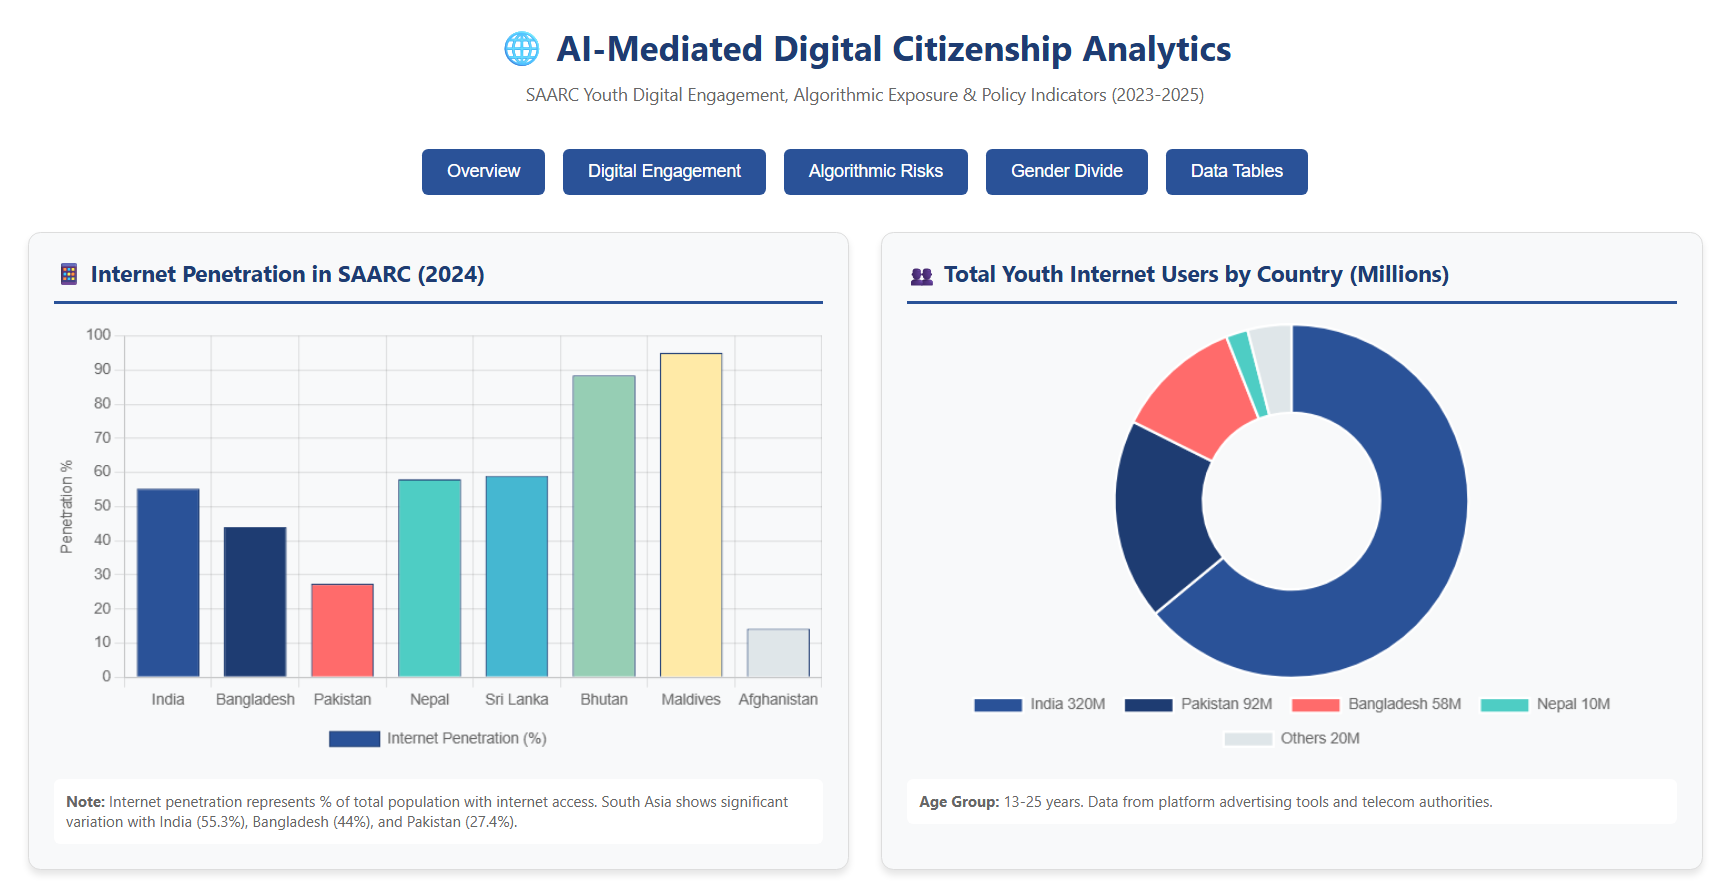
\includegraphics[width=0.9\textwidth]{figures/ai_dashboard_overview.png}
%   \caption{Dashboard overview interface}
% \end{figure}




\chapter{Baseline Youth Digital Landscape Dashboards}
\label{app:baseline_dashboard}

This appendix documents the baseline descriptive dashboards developed during the initial phase of the research. These dashboards were designed as exploratory visualization instruments to map youth internet access, social media penetration, and digital harm prevalence across South Asian countries prior to introducing AI-mediated analytical layers.

\section{Purpose and Analytical Scope}

The baseline dashboards serve three primary functions. First, they provide a regional snapshot of youth digital access patterns, highlighting structural inequalities across countries, gender, and age groups. Second, they identify dominant platform ecosystems through which algorithmic exposure occurs, establishing the empirical foundation for later AI-focused analysis. Third, they contextualize digital harms within access conditions, revealing how misinformation, harassment, and privacy risks intersect with shared-device usage and gender disparities.

These dashboards are descriptive rather than predictive and do not model algorithmic behavior directly. Instead, they function as an empirical grounding layer for the applied AI-mediated analytics discussed in Chapter~3.

\section{Dashboard Architecture and Visualization Design}

The dashboards were implemented as interactive, browser-based visualizations using HTML, CSS, JavaScript, and the Chart.js library. The system is organized into modular sections covering:

\begin{itemize}
  \item Internet penetration and youth access by country
  \item Gender-based digital access gaps
  \item Social media platform dominance and multi-platform exposure
  \item Prevalence of digital harms affecting youth
  \item Age-wise adoption patterns
  \item Device access inequality, including shared-device usage
\end{itemize}

Interactive charts, summary tables, and contextual annotations were used to support exploratory analysis and policy-oriented interpretation rather than statistical inference.

\section{Data Sources and Methodological Notes}

The dashboards synthesize publicly available secondary data from authoritative international and regional sources, including GSMA Intelligence, UNICEF, UNESCO, DataReportal, WHO, and peer-reviewed academic literature. Values presented represent aggregated indicators intended to illustrate structural patterns rather than precise prevalence estimates. Differences in survey methodology, sampling frames, and reporting periods across sources may introduce variation.

\section{Research Role and Limitations}

While the dashboards offer valuable regional insight, they do not access proprietary platform data or internal algorithmic metrics. As such, they cannot directly observe recommendation system behavior. This limitation motivated the development of simulation-based and AI-driven analytical tools presented later in the study.

Together, the baseline dashboards and subsequent computational extensions demonstrate a layered research approach, progressing from descriptive mapping to mechanism-oriented analysis of AI-mediated digital citizenship.

\section{Access Links}
\begin{itemize}
  \item Live Deployment \href{https://south-asian-youth-digital-landscape.netlify.app/}{(Netlify):} \textit{https://south-asian-youth-digital-landscape.netlify.app/}
  \item Source Code \href{https://github.com/Kartik-Kashyap/SAARC-internship-research-work/tree/main/(web)SA\_youth\_digital\_analysis\_dashboard}{(GitHub Repository):} \textit{https://github.com/Kartik-Kashyap/SAARC-internship-research-work/tree/main/(web)SA\_youth\_digital\_analysis\_dashboard}
\end{itemize}




\chapter{Echo Chamber and Polarization Simulator}
\label{app:echo_simulator}

This appendix documents the Echo Chamber and Polarization Simulator developed as part of this research. The simulator serves as a conceptual and pedagogical tool to demonstrate how polarization and echo chambers can emerge from the interaction of cognitive biases, social network structure, and algorithmic amplification.

\section{Purpose and Scope}

The simulator was designed to:
\begin{itemize}
    \item Illustrate theoretical models of opinion dynamics discussed in the literature
    \item Isolate causal mechanisms that are difficult to observe on real social media platforms
    \item Provide an interactive demonstration for educational and policy-oriented interpretation
\end{itemize}

The model does not aim to replicate proprietary platform algorithms or predict real-world behavior. Instead, it functions as an explanatory abstraction consistent with established computational social science approaches.

\section{Model Structure}

The simulation represents users as agents holding continuous opinions on a normalized scale between 0 and 1. Each agent interacts with others according to the following mechanisms:

\begin{itemize}
    \item \textbf{Bounded Confidence:} Agents only influence each other when opinion differences fall below a tolerance threshold.
    \item \textbf{Homophily:} Network connections are probabilistically biased toward agents with similar opinions.
    \item \textbf{Algorithmic Amplification:} A parameterized force shifts opinions toward extremes, simulating engagement-optimized recommendation dynamics.
\end{itemize}

The model tracks polarization, opinion clustering, and information diversity over multiple simulation steps.

\section{Key Metrics}

The simulator computes several aggregate indicators:
\begin{itemize}
    \item Opinion variance as a measure of polarization
    \item Number of distinct opinion clusters
    \item Entropy-based information diversity
    \item Within-group versus between-group opinion distances
\end{itemize}

These metrics align with measures commonly used in opinion dynamics and polarization research.

\section{Scenarios}

Predefined scenarios allow comparison between:
\begin{itemize}
    \item Baseline conditions (cognitive, social, and algorithmic effects combined)
    \item Absence of algorithmic amplification
    \item Algorithmic amplification without social filtering
    \item High-polarization extreme conditions
\end{itemize}

Comparative visualization highlights how algorithmic mechanisms accelerate and stabilize polarization.

\section{Implementation}

\begin{itemize}
    \item Frontend: HTML, CSS, JavaScript
    \item Visualization: Chart.js
    \item Model Type: Rule-based agent simulation
\end{itemize}

\section{Access}

\begin{itemize}
    \item Live Demonstration \href{https://centrifuge-polarization-simulator.netlify.app/}{(Netlify):} \textit{https://centrifuge-polarization-simulator.netlify.app/}
    \item Source Code \href{https://github.com/Kartik-Kashyap/SAARC-internship-research-work/tree/main/\%28web\%29centrifuge_mathematical_echo_chamber_simulation}{(GitHub Repository):} \textit{https://github.com/Kartik-Kashyap/SAARC-internship-research-work/tree/main/\%28web\%29centrifuge\_mathematical\_echo\_chamber\_simulation}
\end{itemize}

\section{Limitations}

The simulator intentionally simplifies real-world conditions. It assumes homogeneous user behavior, static parameters, and a single opinion dimension. These limitations are consistent with its explanatory purpose and do not undermine its value as a conceptual demonstration of algorithmic and social interaction effects.


\chapter{Rule-Based Feed Simulator}
\label{app:rule_based_simulator}

This appendix documents the design, rationale, and implementation of the Rule-Based Feed Simulator developed as part of this study. Unlike the AI-driven feed simulator discussed in Chapter~3, this system does not employ machine learning or generative models. Instead, it relies on deterministic logic and predefined scoring rules to demonstrate how algorithmic feedback loops can emerge even in the absence of artificial intelligence.

\section{Purpose and Research Rationale}

The Rule-Based Feed Simulator was developed to serve three primary research objectives. First, it provides a transparent and interpretable demonstration of algorithmic amplification mechanisms without reliance on opaque AI models. Second, it functions as an educational tool, enabling policymakers, educators, and students to observe how engagement-driven personalization operates through simple conditional logic. Third, it establishes a conceptual baseline against which the added risks and power asymmetries of AI-driven personalization can be compared.

By isolating feedback dynamics from probabilistic or generative behavior, the simulator demonstrates that echo chambers, dopamine loops, and content narrowing are not exclusive consequences of advanced artificial intelligence but can arise from basic engagement optimization strategies.

\section{System Overview}

The simulator models a simplified social media feed composed of predefined post categories, including:

\begin{itemize}
  \item Polarizing political content
  \item Shallow or viral content
  \item Educational or analytical content
  \item Balanced or multi-perspective content
\end{itemize}

Each post is assigned fixed impact values across four digital citizenship dimensions:
\begin{enumerate}
  \item Attention span
  \item Polarization index
  \item Critical thinking capacity
  \item Informational diversity
\end{enumerate}

User interactions (clicks or consumption events) incrementally update these metrics according to deterministic rules. Subsequent content recommendations are conditionally selected based on cumulative interaction scores rather than learned representations.

\section{Algorithmic Logic and Scoring Rules}

The recommendation mechanism follows a rule-based prioritization model:

\begin{itemize}
  \item Content categories previously engaged with receive increased selection probability.
  \item High-frequency engagement with emotionally salient content reduces attention and diversity metrics.
  \item Repeated interaction with polarizing content increases polarization scores and narrows future recommendations.
  \item Engagement with educational or balanced content partially restores cognitive and diversity metrics.
\end{itemize}

This logic mirrors engagement-based ranking strategies observed in real-world platforms, while remaining fully interpretable and auditable.

\section{Educational and Policy Relevance}

From a policy and digital literacy perspective, the rule-based simulator offers two key advantages. First, it allows stakeholders to observe harmful dynamics without attributing outcomes to artificial intelligence alone, reinforcing the argument that governance must address incentive structures rather than technology labels. Second, its deterministic nature makes it suitable for classroom instruction, workshops, and public demonstrations where transparency is essential.

The simulator has been intentionally designed to avoid persuasive optimization or adaptive manipulation. Its purpose is illustrative, not behavioral intervention or prediction.

\section{Deployment and Accessibility}

As the system does not rely on external APIs or local AI models, it has been deployed as a static web application for public access and demonstration purposes.

\begin{itemize}
  \item \textbf{Live Demo \href{https://social-media-echo-chamber-simulator.netlify.app/}{(Netlify)}} \textit{https://social-media-echo-chamber-simulator.netlify.app/}
  \item \textbf{Source Code \href{https://github.com/Kartik-Kashyap/SAARC-internship-research-work/tree/main/(web)echo-chamber-hard-coded-simulator}{(GitHub):}} \textit{https://github.com/Kartik-Kashyap/SAARC-internship-research-work/tree/main/(web)echo-chamber-hard-coded-simulator}
\end{itemize}

The deployed version enables real-time interaction and visualization of metric changes, supporting its use in educational and policy-oriented contexts.

\section{Relationship to AI-Based Feed Simulator}

This rule-based system complements the AI-driven simulator described in Chapter~3 by providing a controlled baseline. While the AI-based system demonstrates adaptive personalization through large language models, the rule-based simulator establishes that harmful feedback loops can emerge even under fixed, non-learning conditions.

Together, these systems reinforce a central conclusion of this study: algorithmic harm is not solely a function of artificial intelligence but of optimization objectives embedded within digital platforms.



\chapter{AI-Based Social Media Feed Simulator}
\label{app:ai_simulator}

This appendix documents the AI-based social media feed simulator developed to examine adaptive algorithmic personalization and its implications for digital citizenship.

\section{Objective}

The simulator was designed to demonstrate how engagement-optimized algorithms adapt content delivery based on user interaction patterns, and how such adaptation influences attention, polarization, critical thinking, and informational diversity.

\section{System Architecture}

The system consists of:
\begin{itemize}
    \item A frontend interface simulating a social media feed
    \item Behavioral tracking of user interactions
    \item A local backend integrating a large language model (LLaMA 3.2)
    \item A feedback mechanism generating interpretive reports
\end{itemize}

The AI model generates new posts conditioned on dominant content preferences inferred from prior interactions. The model is intentionally instructed to prioritize engagement rather than accuracy or balance.

\section{Content Categories}

Posts are categorized into:
\begin{itemize}
    \item Polarizing political content
    \item Shallow viral content
    \item Dopamine-driven short-form media
    \item Misinformation
    \item Educational analysis
    \item Balanced regional discourse
\end{itemize}

Each category is associated with heuristic impact scores affecting user metrics.

\section{Digital Citizenship Metrics}

The simulator tracks:
\begin{itemize}
    \item Attention span
    \item Polarization index
    \item Critical thinking capacity
    \item Information diversity
\end{itemize}

These metrics are combined into a final Digital Citizenship Report Card presented at the end of each session.

\section{Ethical Design Considerations}

The system does not store personal data, deploy external APIs, or simulate real individuals. Its purpose is pedagogical and analytical. The AI model operates locally to ensure transparency and reproducibility.

\section{Access}

\begin{itemize}
    \item \href{https://github.com/Kartik-Kashyap/SAARC-internship-research-work/tree/main/(AI)social-media-echo-chamber-simulator}{Source Code Repository:} \textit{https://github.com/Kartik-Kashyap/SAARC-internship-research-work/tree/main/(AI)social-media-echo-chamber-simulator}
    \item Local Deployment Instructions: Provided in \texttt{README.md}
\end{itemize}

\section{Limitations}

The simulator abstracts complex platform dynamics into simplified interactions. It does not model economic incentives, advertiser influence, or cross-platform effects. These limitations are consistent with its illustrative purpose.



% =========================
% APPENDIX: SAARC AI
% =========================
\chapter{SAARC AI: System Design and Constraint Architecture}
\label{app:saarc_ai}

This appendix documents the technical and design foundations of the SAARC AI assistant developed during this study. The system is presented not as a commercial conversational agent, but as a constrained, value-aligned artificial intelligence designed for regional sensemaking and educational use.

\section{Design Objectives}
\begin{itemize}
  \item Domain-restricted knowledge scope (SAARC-only)
  \item Neutral, diplomatic, and multi-perspective responses
  \item Explicit refusal of divisive, non-regional, or inflammatory queries
\end{itemize}

% =====================================================
% CONCISE APPENDIX F: SAARC AI SYSTEM DOCUMENTATION
% Replace sections F.2 and F.3 with this content
% =====================================================

\section{System Prompt and Constraint Logic}

The SAARC AI Assistant operates under strict domain constraints enforced through system-level instructions. The core system prompt, embedded in each API request, defines operational boundaries and refusal mechanisms:

\begin{lstlisting}[language=Python, caption={SAARC AI Core System Prompt}, basicstyle=\ttfamily\scriptsize, breaklines=true]
You are the SAARC AI Assistant, an expert on the South 
Asian Association for Regional Cooperation (SAARC) and 
its member nations.

SAARC Member Countries: Afghanistan, Bangladesh, Bhutan, 
India, Maldives, Nepal, Pakistan, Sri Lanka

YOUR ROLE:
- Answer questions ONLY about SAARC nations, regional 
  cooperation, culture, history, diplomacy, and economics
- Be informative, balanced, and diplomatic
- Promote understanding between SAARC nations
- Avoid political bias or favoritism
- Present multiple perspectives on contentious issues

STRICT RESTRICTIONS:
- Decline questions unrelated to SAARC or South Asia
- Never answer offensive or inflammatory questions
- Do not take sides in conflicts
- Refuse divisive or hateful content

TONE: Professional, warm, respectful. Use South Asian 
greetings (Namaste, Salaam) appropriately.
\end{lstlisting}

\subsection{Constraint Enforcement Mechanisms}

The system implements three enforcement layers:

\begin{enumerate}
    \item \textbf{Topic Filtering:} Queries outside SAARC scope are politely declined with explanation.
    \item \textbf{Tone Policing:} Inflammatory or divisive content is systematically refused.
    \item \textbf{Diplomatic Neutrality:} The system avoids favoritism and presents balanced perspectives.
\end{enumerate}

This prompt-based architecture prioritizes transparency and educational purpose over engagement optimization, demonstrating how institutional constraints can be embedded within AI systems through design rather than post-hoc moderation.

% =====================================================

\section{Model Deployment and Local Execution}

The system utilizes LLaMA 3.2 (3B parameters) deployed locally via Ollama, ensuring complete data privacy and transparency.

\subsection{Technology Stack}

\begin{itemize}
    \item \textbf{Frontend:} React with Tailwind CSS, Lucide icons
    \item \textbf{AI Backend:} Ollama serving LLaMA 3.2 (3B)
    \item \textbf{Communication:} HTTP POST to \texttt{localhost:11434/api/generate}
\end{itemize}

\subsection{System Requirements}

\begin{table}[H]
\centering
\caption{Deployment Requirements}
\begin{tabular}{lll}
\toprule
\textbf{Component} & \textbf{Minimum} & \textbf{Recommended} \\
\midrule
RAM & 8 GB & 16 GB \\
Storage & 5 GB & 10 GB \\
Processor & 4-core CPU & 8-core CPU / GPU \\
\bottomrule
\end{tabular}
\end{table}

\subsection{Installation Procedure}

\subsubsection{Step 1: Install Ollama and Model}
\begin{lstlisting}[language=bash, caption={Ollama Setup}]
# Install Ollama
curl https://ollama.ai/install.sh | sh
# Download LLaMA 3.2 (approx. 2GB)
ollama pull llama3.2
# Start service (runs on localhost:11434)
ollama serve
\end{lstlisting}

\subsubsection{Step 2: Deploy Frontend}
\begin{lstlisting}[language=bash, caption={React Application Setup}]
# Clone repository
git clone https://github.com/Kartik-Kashyap/\
SAARC-internship-research-work.git
cd SAARC-internship-research-work/\(AI\)SAARC-AI-Assistant

# Install dependencies and run
npm install
npm run dev
# Access at http://localhost:5173
\end{lstlisting}

\subsection{API Communication Structure}

The frontend transmits user queries via HTTP POST:

\begin{lstlisting}[language=JavaScript, caption={API Request Implementation}, basicstyle=\ttfamily\scriptsize]
const response = await fetch('http://localhost:11434/api/generate', {
  method: 'POST',
  headers: { 'Content-Type': 'application/json' },
  body: JSON.stringify({
    model: 'llama3.2',
    prompt: `${systemPrompt}\n\nUser: ${userInput}\n\nAssistant:`,
    stream: false
  })
});
const data = await response.json();
\end{lstlisting}

Response latency ranges from 2--8 seconds depending on hardware (faster with GPU acceleration).

\subsection{Data Privacy}

Local deployment ensures:
\begin{itemize}
    \item No external data transmission
    \item No conversation logging or analytics
    \item Complete user control over inference
    \item Suitable for educational and research contexts
\end{itemize}

\subsection{Troubleshooting}

\textbf{Connection Error:} Verify Ollama is running (\texttt{ollama serve}) and accessible at \texttt{localhost:11434}.

\textbf{Slow Responses:} Close resource-intensive applications, increase RAM allocation, or enable GPU acceleration.

\textbf{Model Not Found:} Confirm installation with \texttt{ollama list}; re-download if necessary.

% =====================================================
% END OF CONCISE APPENDIX F
% =====================================================

\section{Interface Design and User Interaction}
The user interface was designed for clarity and accessibility, emphasizing a clean workspace for research. 

\section{Interface Design and User Interaction}
The user interface was designed for clarity and accessibility, emphasizing a clean workspace for research. The following figures illustrate the system's operational environment and its multilingual capabilities.

\begin{figure}[H]
    \centering
    % First Screenshot: Main Interface (Full Width)
    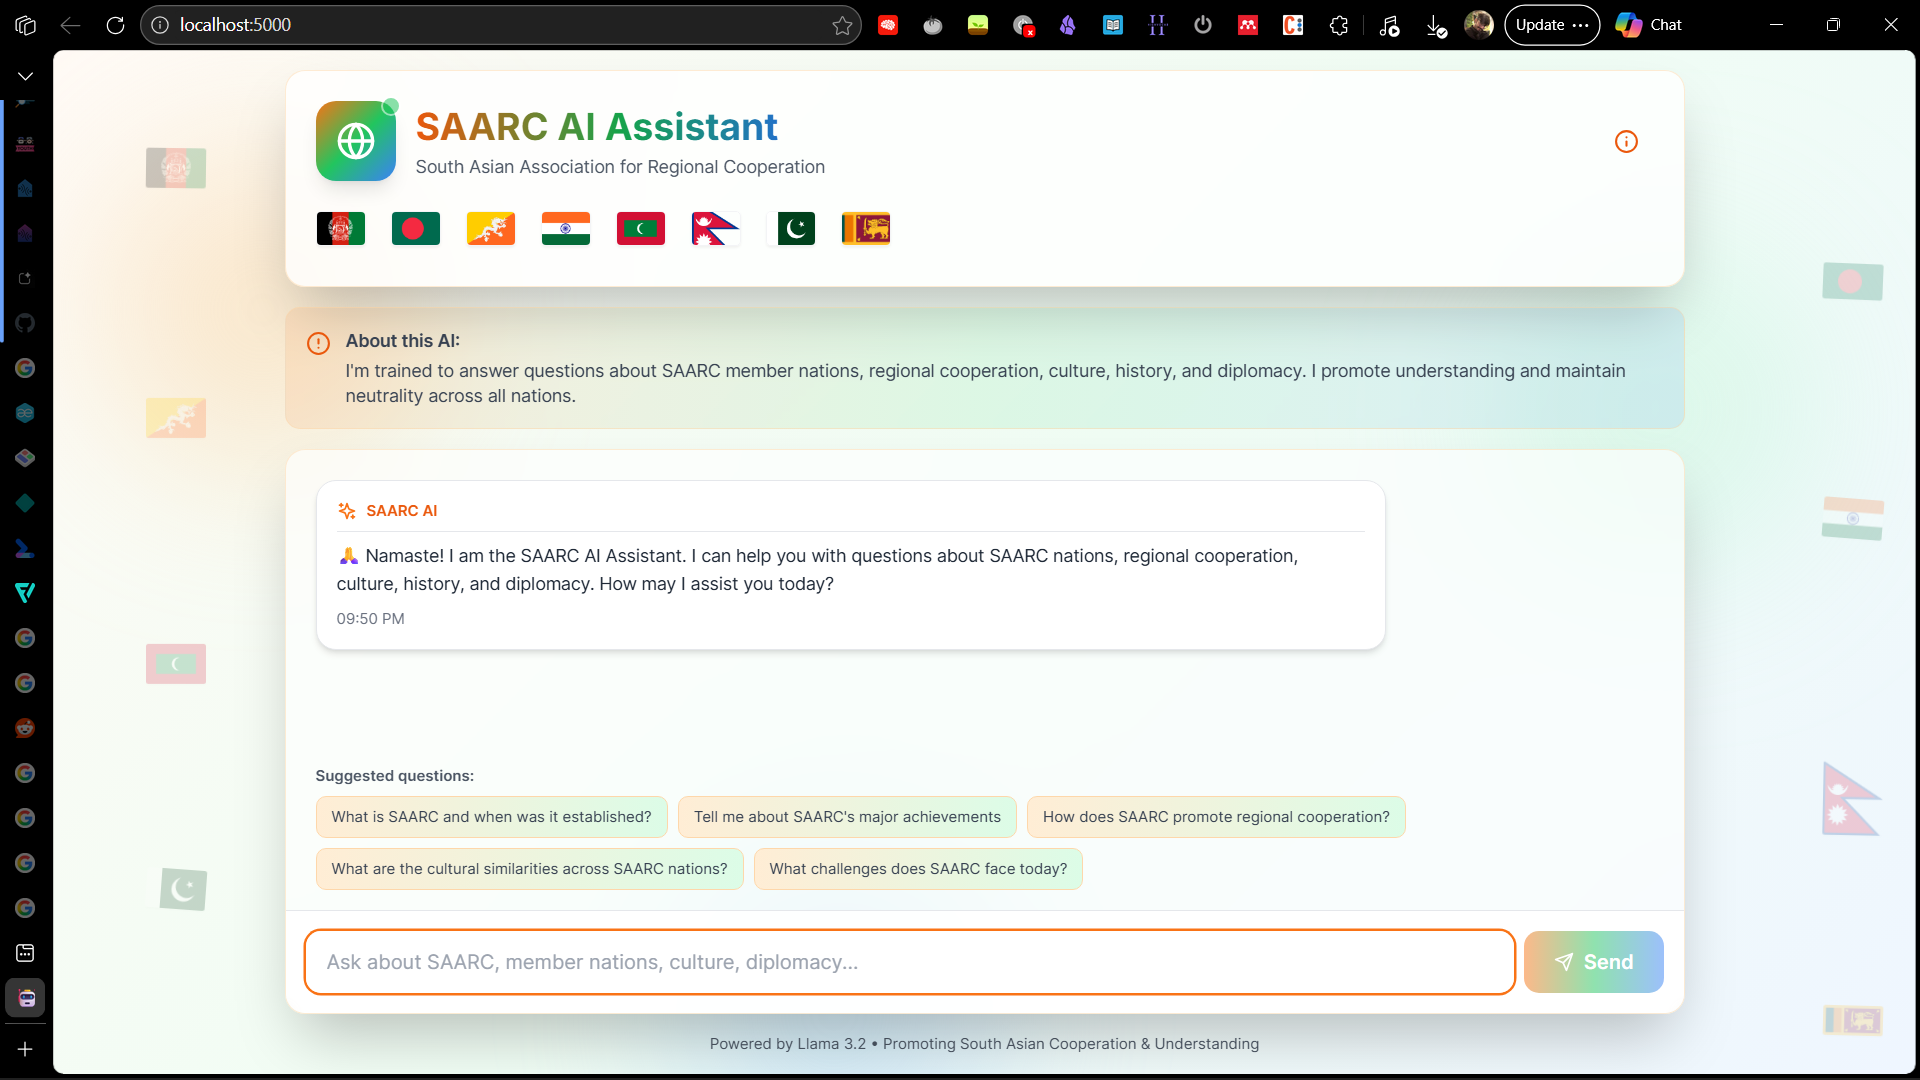
\includegraphics[width=1\textwidth]{figures/main_interface.png}
    \caption{SAARC AI Main Opening Interface (Desktop View).}
    \label{fig:saarc_ui_main}
    
    \vspace{1.5em} % Adds some breathing room between the two images

    % Second Screenshot: Hindi Interaction (0.8 Width)
    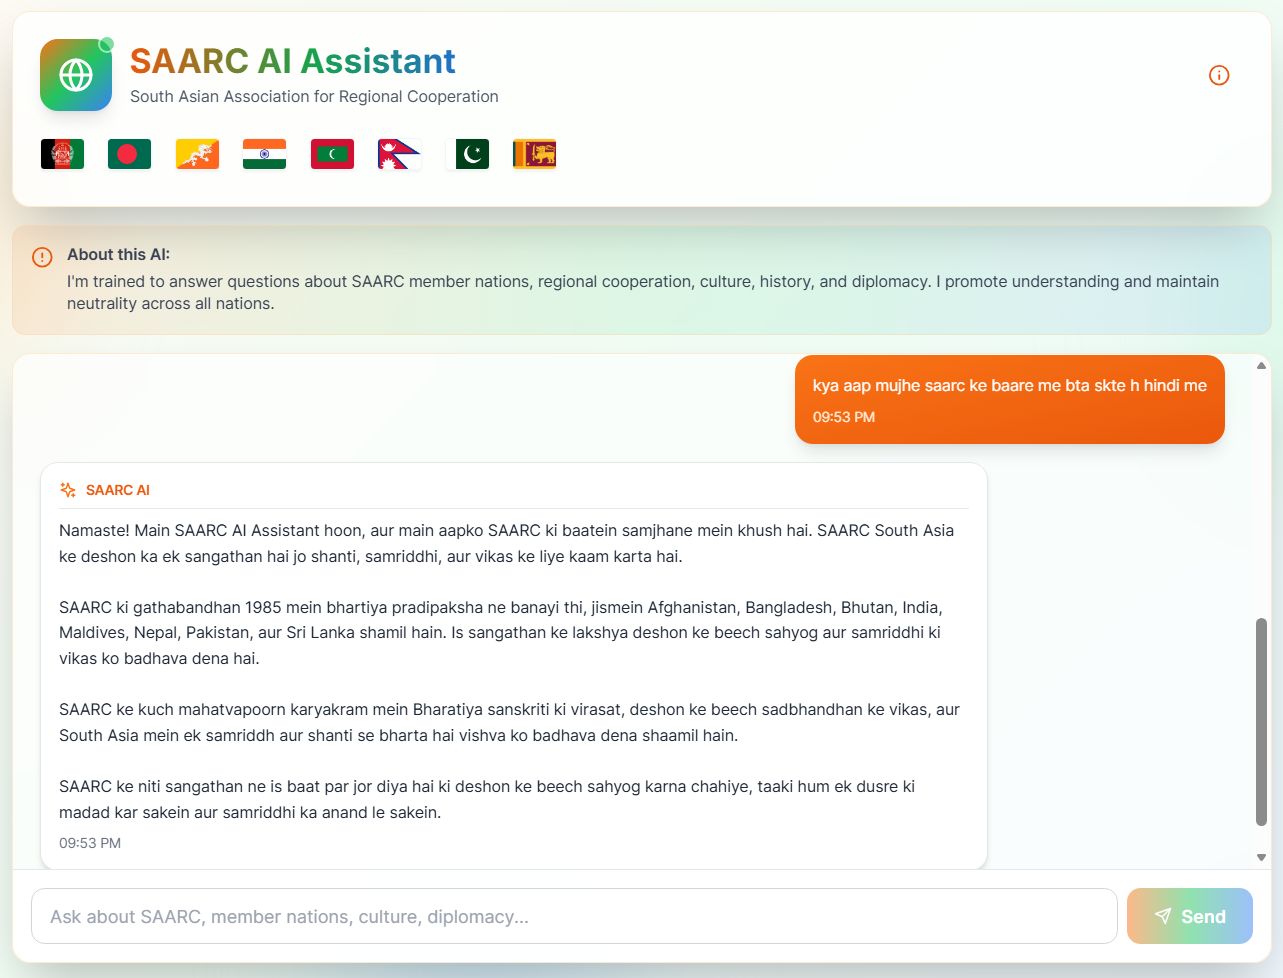
\includegraphics[width=0.8\textwidth]{figures/hindi_chat.png} 
    \caption{Multilingual support: Interaction and response in Hindi.}
    \label{fig:saarc_ui_hindi}
\end{figure}

As shown in Figure~\ref{fig:saarc_ui_hindi}, the model maintains its persona and constraints across regional languages, demonstrating its capability to serve a diverse linguistic population while remaining within its defined geopolitical knowledge boundaries.

\section{Limitations}
This system does not claim completeness, real-time geopolitical accuracy, or policy authority. Its purpose is illustrative and educational, demonstrating how institutional constraints reshape AI behavior.

\section{Access}

\begin{itemize}
    \item \href{https://github.com/Kartik-Kashyap/SAARC-internship-research-work/tree/main/(AI)SAARC-AI-Assistant}{Source Code Repository:} \textit{https://github.com/Kartik-Kashyap/SAARC-internship-research-work/tree/main/(AI)SAARC-AI-Assistant}
    \item Local Deployment Instructions: Provided in \texttt{README.md}
\end{itemize}


% =========================
% REFERENCES
% =========================
\newpage
\nocite{*}
% \bibliographystyle{apacite}
% % The command below tells apacite to handle the TOC entry automatically
% \renewcommand{\bibliographytypesize}{\normalsize}
% \bibliography{references}
\printbibliography[title={References}]

\end{document}
